\documentclass{article}
\usepackage{graphicx} % Required for inserting images
\graphicspath{ {figures/} }
\usepackage{array}
\usepackage{float}
\usepackage{caption}
\usepackage{amsmath}
\usepackage{amsfonts}
\newcommand{\C}{{\mathbb C}}
\newcommand{\E}{{\mathbb E}}
\newcommand{\R}{{\mathbb R}}
\newcommand{\Prr}{{\mathbb P}}
\newcommand{\N}{{\mathbb N}}
\newcommand{\D}{{\mathbb D}}
\newcommand{\Z}{{\mathbb Z}}
\usepackage{hyperref}
\usepackage{pgfplotstable}
\pgfplotsset{compat=1.18}
\usepackage{booktabs}
\usepackage{array}
\usepackage{colortbl}
\usepackage{diagbox}
\usepackage{amsthm}
\newtheorem{theorem}{Theorem}[section]
\newtheorem{lemma}[theorem]{Lemma}
\newtheorem{remark}{Remark}
\newtheorem{note}{Note}[section]
\newtheorem{proposition}{Proposition}
\usepackage{bm}

% Redefine the format for figure captions
\captionsetup[figure]{
    labelfont={bf},   % Make the label bold (e.g., "Figure 1")
    labelsep=colon,   % Set the separator after the label (optional, default is a colon)
}


\title{Term Structure of Firm Characteristics and Multi-Horizon Investment: Tensor Model Interpretability}
% \author{Serhiy Kozak, Markus Pelger, Ye Ye, and James Zhang}
\date{\today}

\begin{document}

\maketitle

\tableofcontents

\listoffigures

\newpage

\section{Economic Interpretation}

In this section, we do not yet discuss results of the tensor model as a pricing model or a multihorizon investor; 
we are setting the foundation with a solid economic interpretation and understanding of the model. In this section, all
components of the model are estimated on the full-sample, unless other specified in a Generalized Canonical Correlation Analysis (GCCA). 


\subsection{An (Interpretable) Univariate Factor Model}

Recall that $L = 1$ is a simple factor model where no lagged characteristics are used. There is extensive research on this. 
We also want to understand what happens when $N = 1$ ie. we have a single-characteristic factor model $\implies$
this is essentially just a PCA on the lagged value portfolios, but it omits an interesting formula, some useful intuition, and a nice equivalence 
that we can establish before talking about the differences between PCA and CP in the next section. In fact, the formula becomes relevant if we impose orthogonality in the time series factors dimension. 

\begin{itemize}
    \item SDF weights in this case and the closed-form formula; this just occurs when the factors are orthogonal, 
    but in practice with more characteristics, the modeling becomes complex and the factors are not orthogonal. Actually, if we impose orthogonality
    in mode $0$ ie. the factors mode, then we can obtain a nice formula even in the case with all characteristics
    \begin{align}
        \omega^S = \left( \left( \sum_{l=1}^S W_l W_l^\top\right) \cdot \text{Var}_t(F_t) \right)^{-1} \text{diag}\left(\sum_{l=1}^S W_l \right) \mathbb{E}_t [F_t]\\
    \end{align}
    If time series factors are orthogonal, then this formula simplifies greatly ie. 
    \begin{align*}
        \omega^S &= \left( \sum_{l=1}^S \text{diag}(W_l \cdot \text{diag}(\text{Var}_t(F_t)) \cdot W_l) \right)^{-1}  \left( \sum_{l=1}^S W_l \cdot \mathbb{E}_t [F_t]\right)\\
        &= \dfrac{\bar{F}_t \cdot \sum_{l=1}^S W_l}{\text{diag}(\text{Var}_t(F_t)) \cdot \sum_{l=1}^S W_l^2}
    \end{align*}
    This simplified formula arises due to the fact that correlations, and thus covariances, between factors is $0$ which allows our 
    covariance matrix to be orthogonal and easily invertible. 
    \item We rediscover level, slope and curvature for equities $\implies$ show a 2x3 graph of the first 6 factors
\end{itemize}

This model is trying to find the optimal linear combination of lagged \emph{value} portfolios; the high-dimensional model 
is more complex because there are many more interactions between lagged portfolios across characteristics. 

\subsection{A High-Dimensional Tensor Model}

\begin{table}[htbp]
    \centering
    \caption{Explained Variation by Lag (L) in Months and Number of Factors (K)}
\begin{tabular}{c|ccccccccc}
    \hline
    \diagbox{L}{K} & 1 & 2 & 3 & 4 & 5 & 10 & 15 & 20 & 25 \\
    \hline
    36 & 0.290 & 0.520 & 0.680 & 0.724 & 0.757 & 0.841 & 0.874 & 0.894 & 0.907 \\
    60 & 0.312 & 0.527 & 0.671 & 0.716 & 0.742 & 0.820 & 0.853 & 0.874 & 0.888 \\
    90 & 0.323 & 0.524 & 0.655 & 0.699 & 0.724 & 0.795 & 0.834 & 0.854 & 0.869 \\
    120 & 0.325 & 0.517 & 0.635 & 0.680 & 0.704 & 0.772 & 0.814 & 0.836 & 0.850 \\
    \hline
    \end{tabular}
\end{table}

\subsubsection{A Comparison of Latent Factors}

The factors outputted from PARAFAC are of direct interest to us because they encode all time-series information 
necessary to model their dynamics of all portfolios at all lags.

\begin{itemize}
    \item Correlation matrices for $F, W, B$
    \item Cumulative log returns $F$
    \item Factors are highly correlated unlike in PCA
    \item Can address how imposing orthogonality in one mode results in a worse decomposition 
    and how imposing non-negativity on the $W$ matrix also results in worse multihorizon Sharpe Ratios (maybe leave this for Appendix?). 
\end{itemize}

\begin{figure}[H]
    \centering
    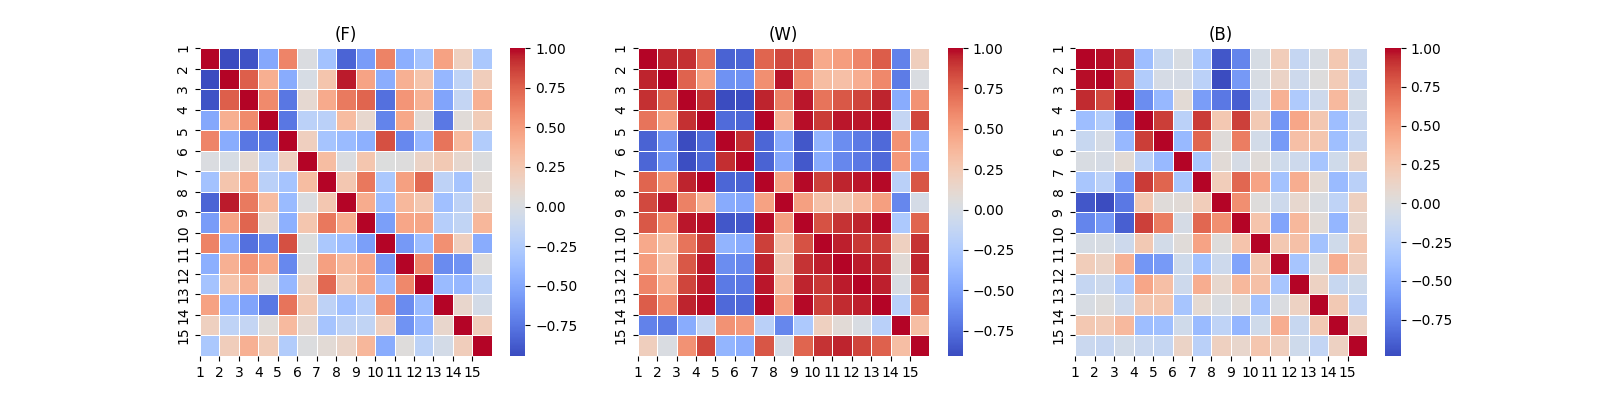
\includegraphics[width=1\linewidth]{corr.png}
    \caption{Correlation Matrices of \bm{$F, W, B$}}
    \label{fig:corr}
\end{figure}

\subsubsection{Cross-Sectional Loadings}

\begin{itemize}
    \item We can potentially impose penalties on $\bm{B}$ to impose sparsity on the loadings on factors to faciliate interpretation $\implies$ 
    similar to Sparse PCA approaches
\end{itemize}

\begin{figure}[H]
    \centering
    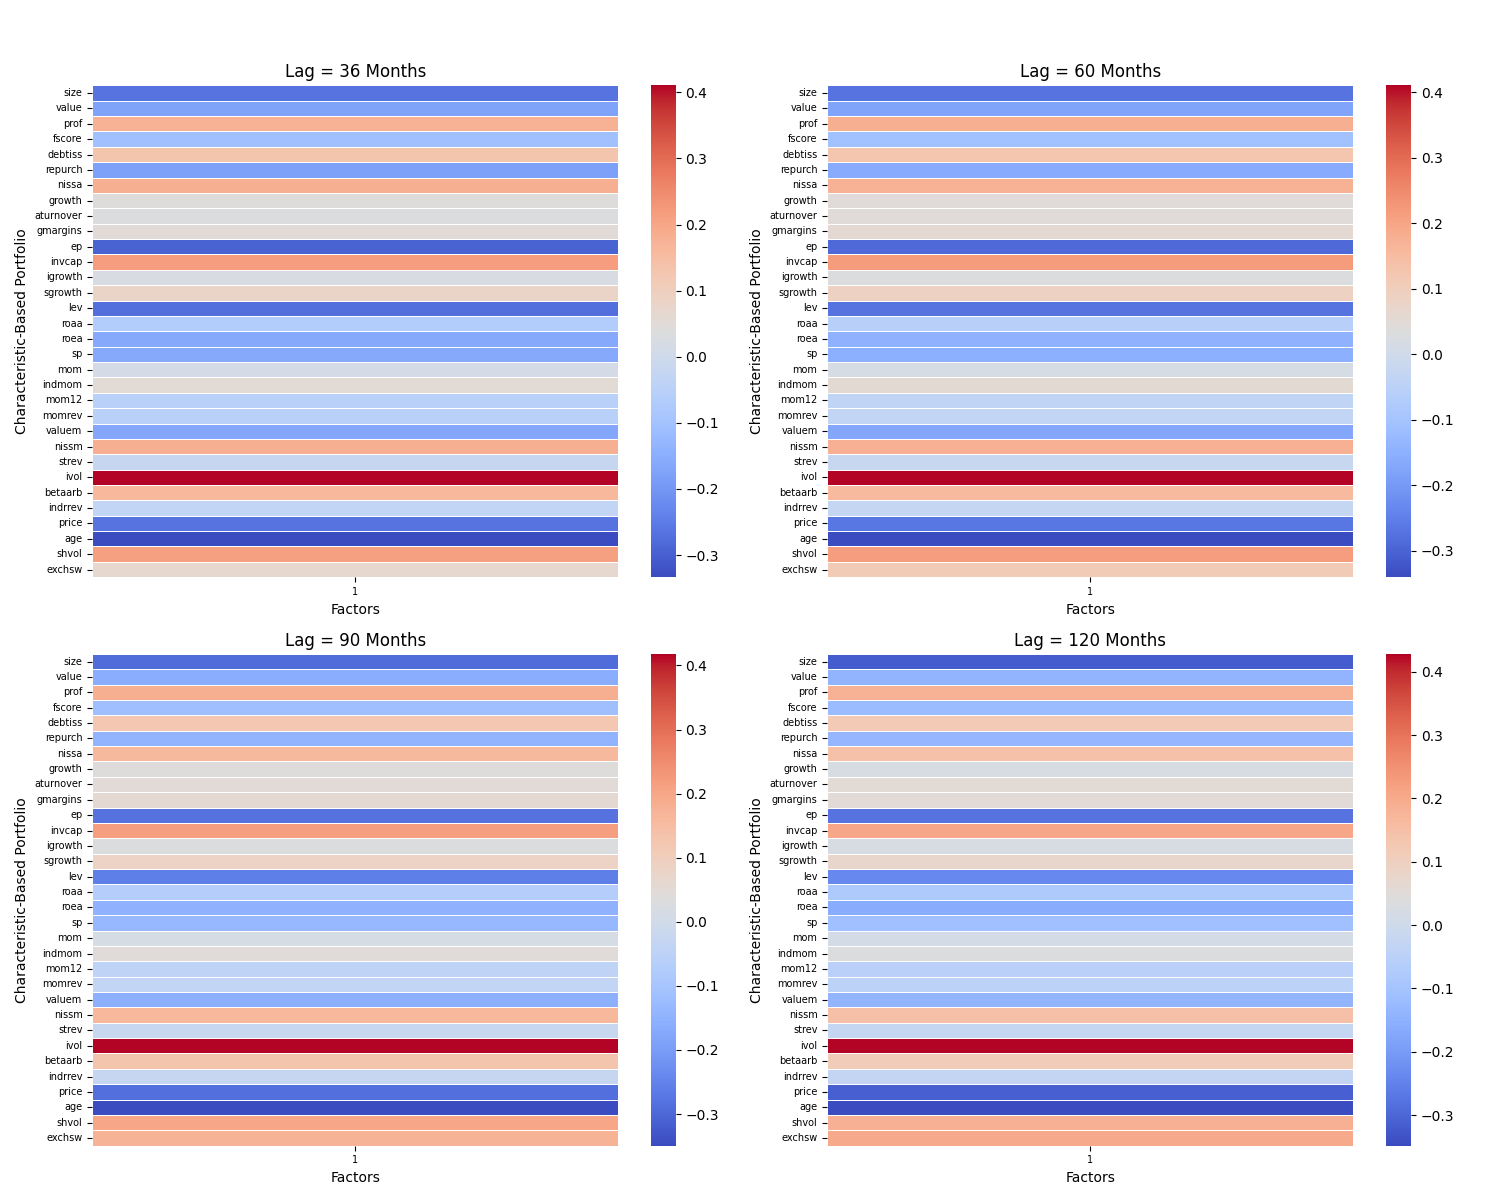
\includegraphics[width=0.85\linewidth]{B_1.png}
    \caption{Cross-Sectional Loadings, K = 1}
    \label{fig:B_1}
\end{figure}
\begin{figure}[H]
    \centering
    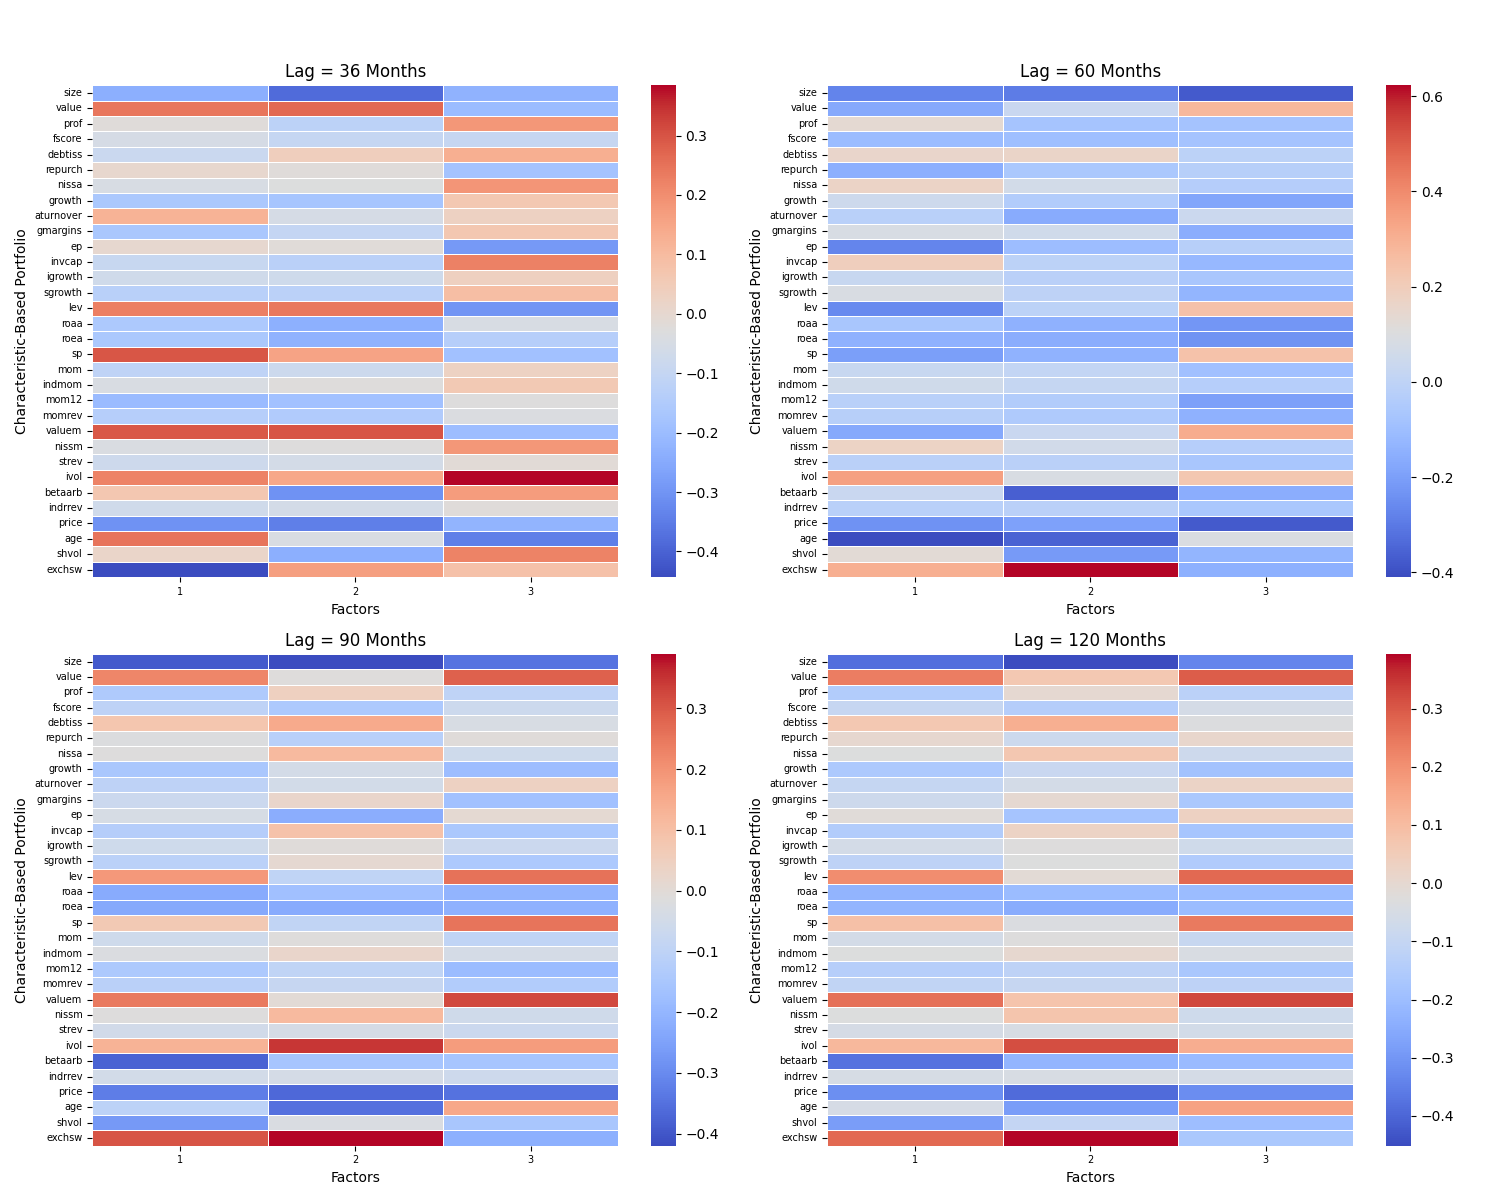
\includegraphics[width=0.85\linewidth]{B_3.png}
    \caption{Cross-Sectional Loadings, K = 3}
    \label{fig:B_3}
\end{figure}
\begin{figure}[H]
    \centering
    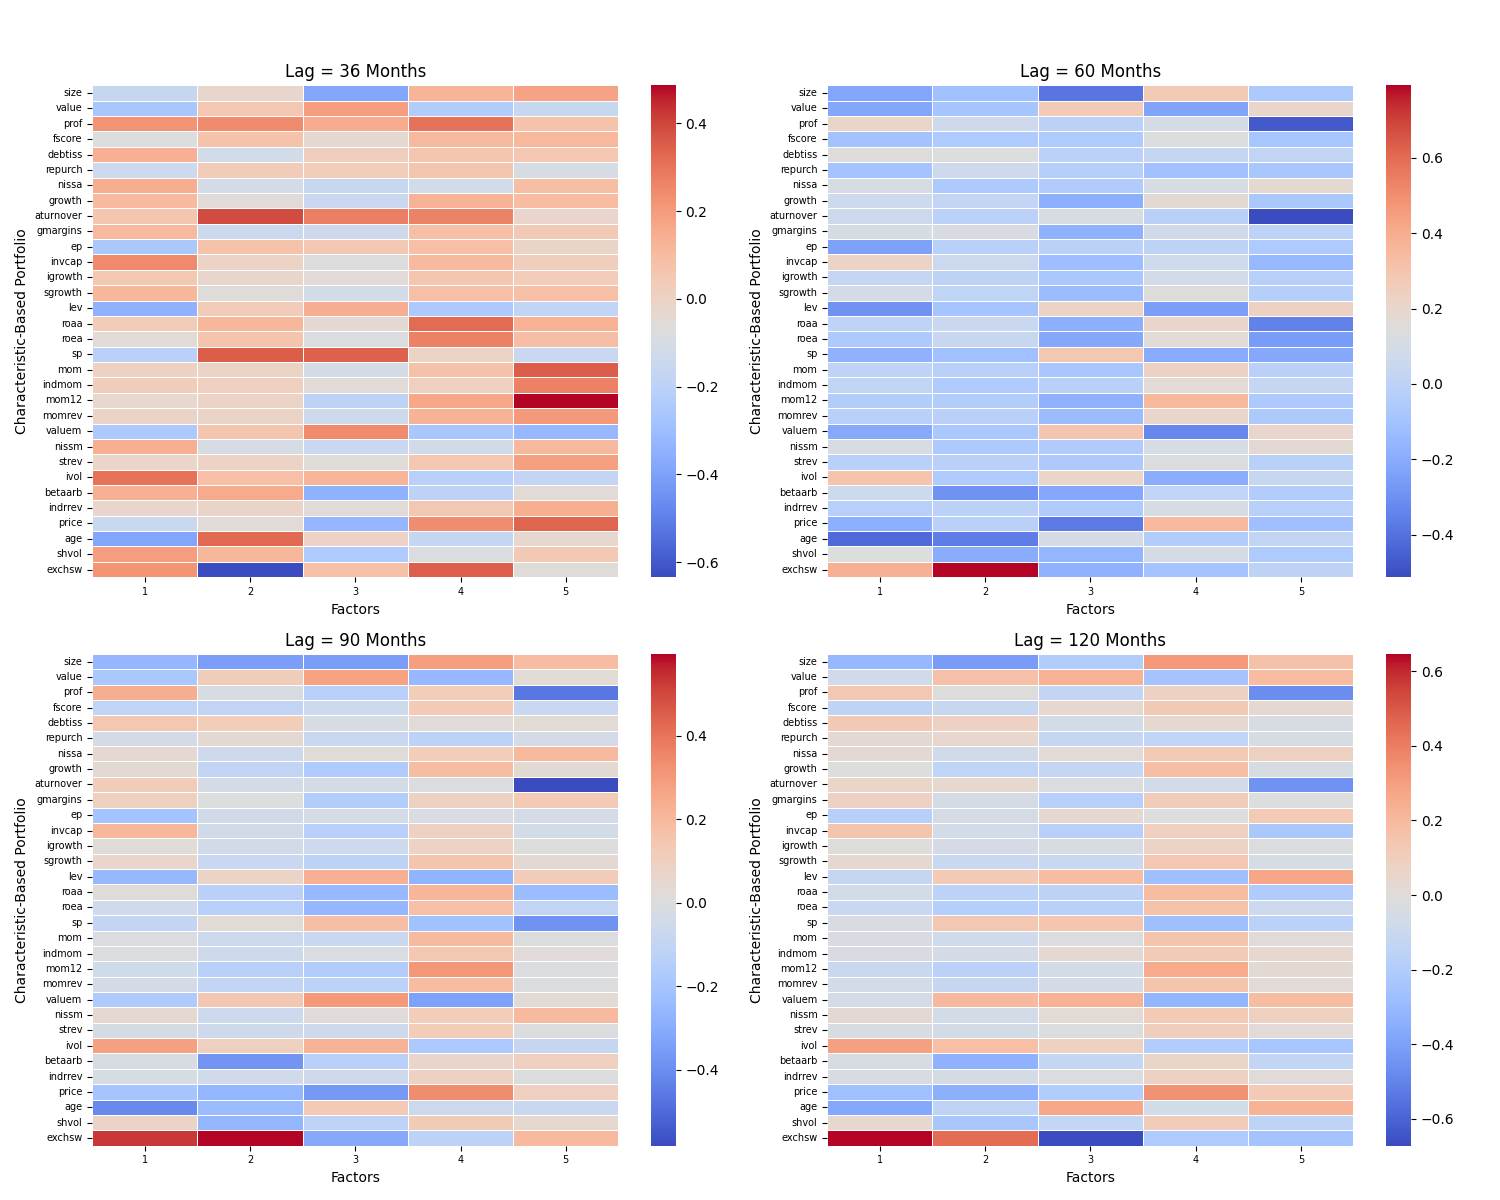
\includegraphics[width=0.85\linewidth]{B_5.png}
    \caption{Cross-Sectional Loadings, K = 5}
    \label{fig:B_5}
\end{figure}
\begin{figure}[H]
    \centering
    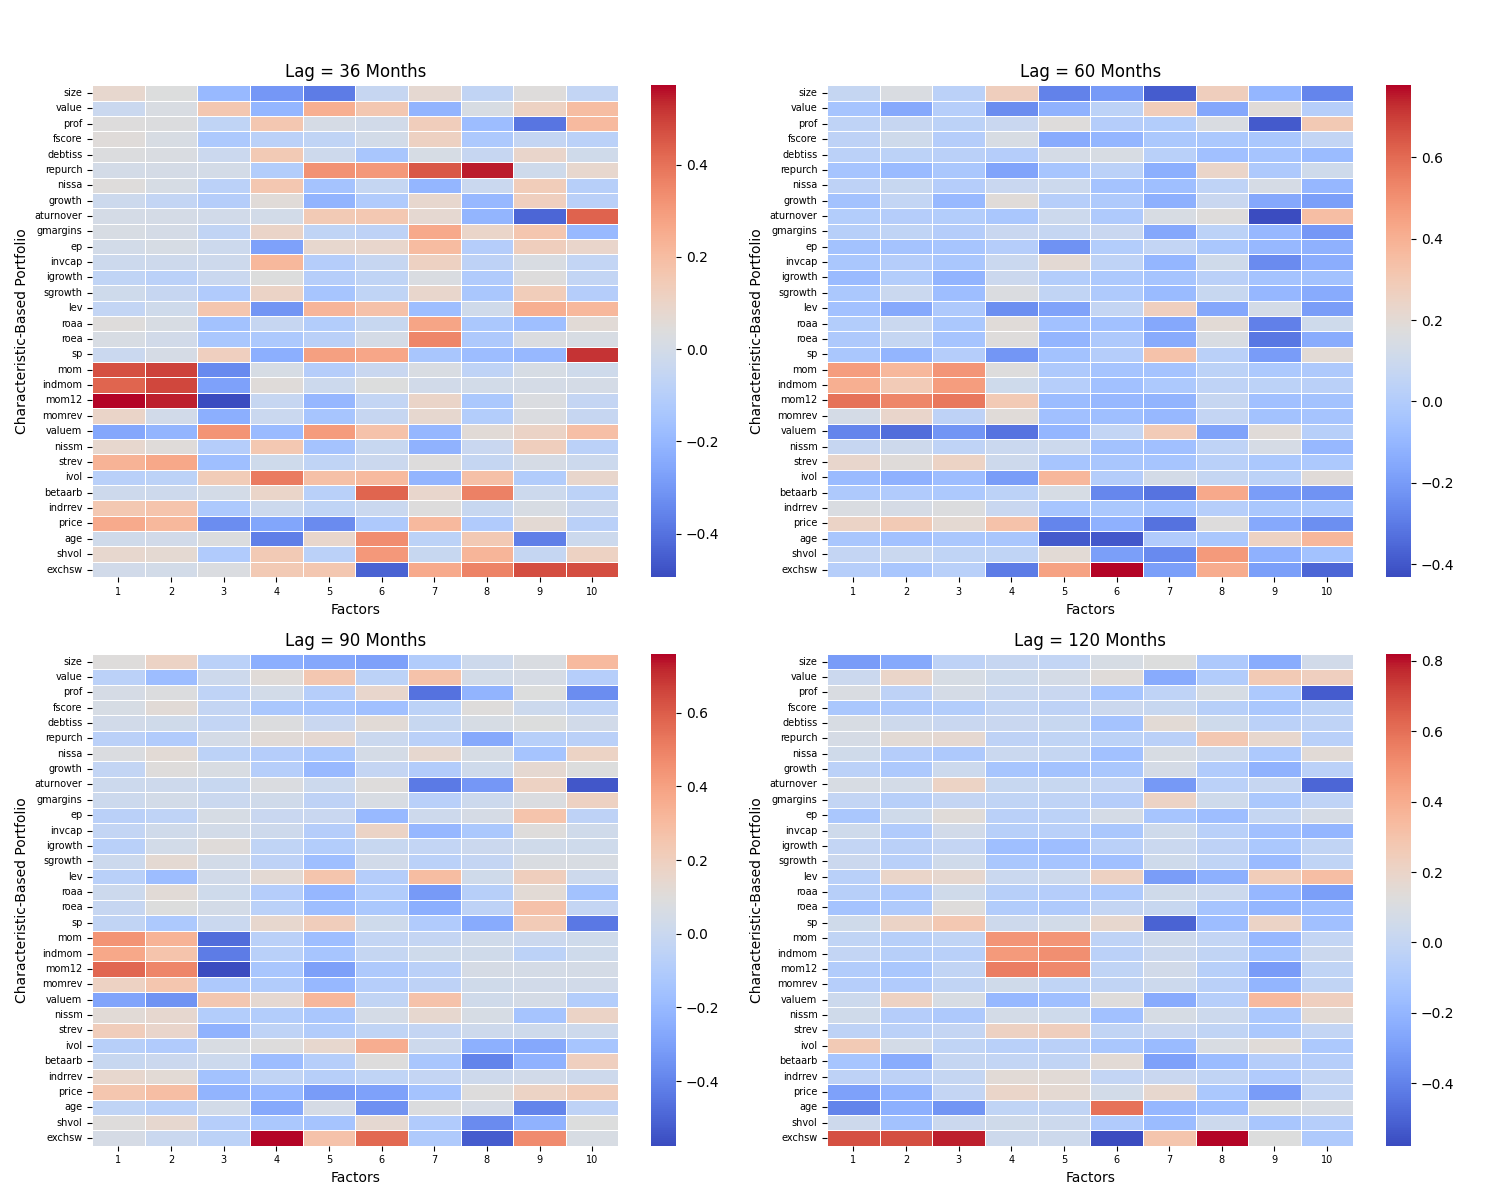
\includegraphics[width=0.85\linewidth]{B_10.png}
    \caption{Cross-Sectional Loadings, K = 10}
    \label{fig:B_10}
\end{figure}
\begin{figure}[H]
    \centering
    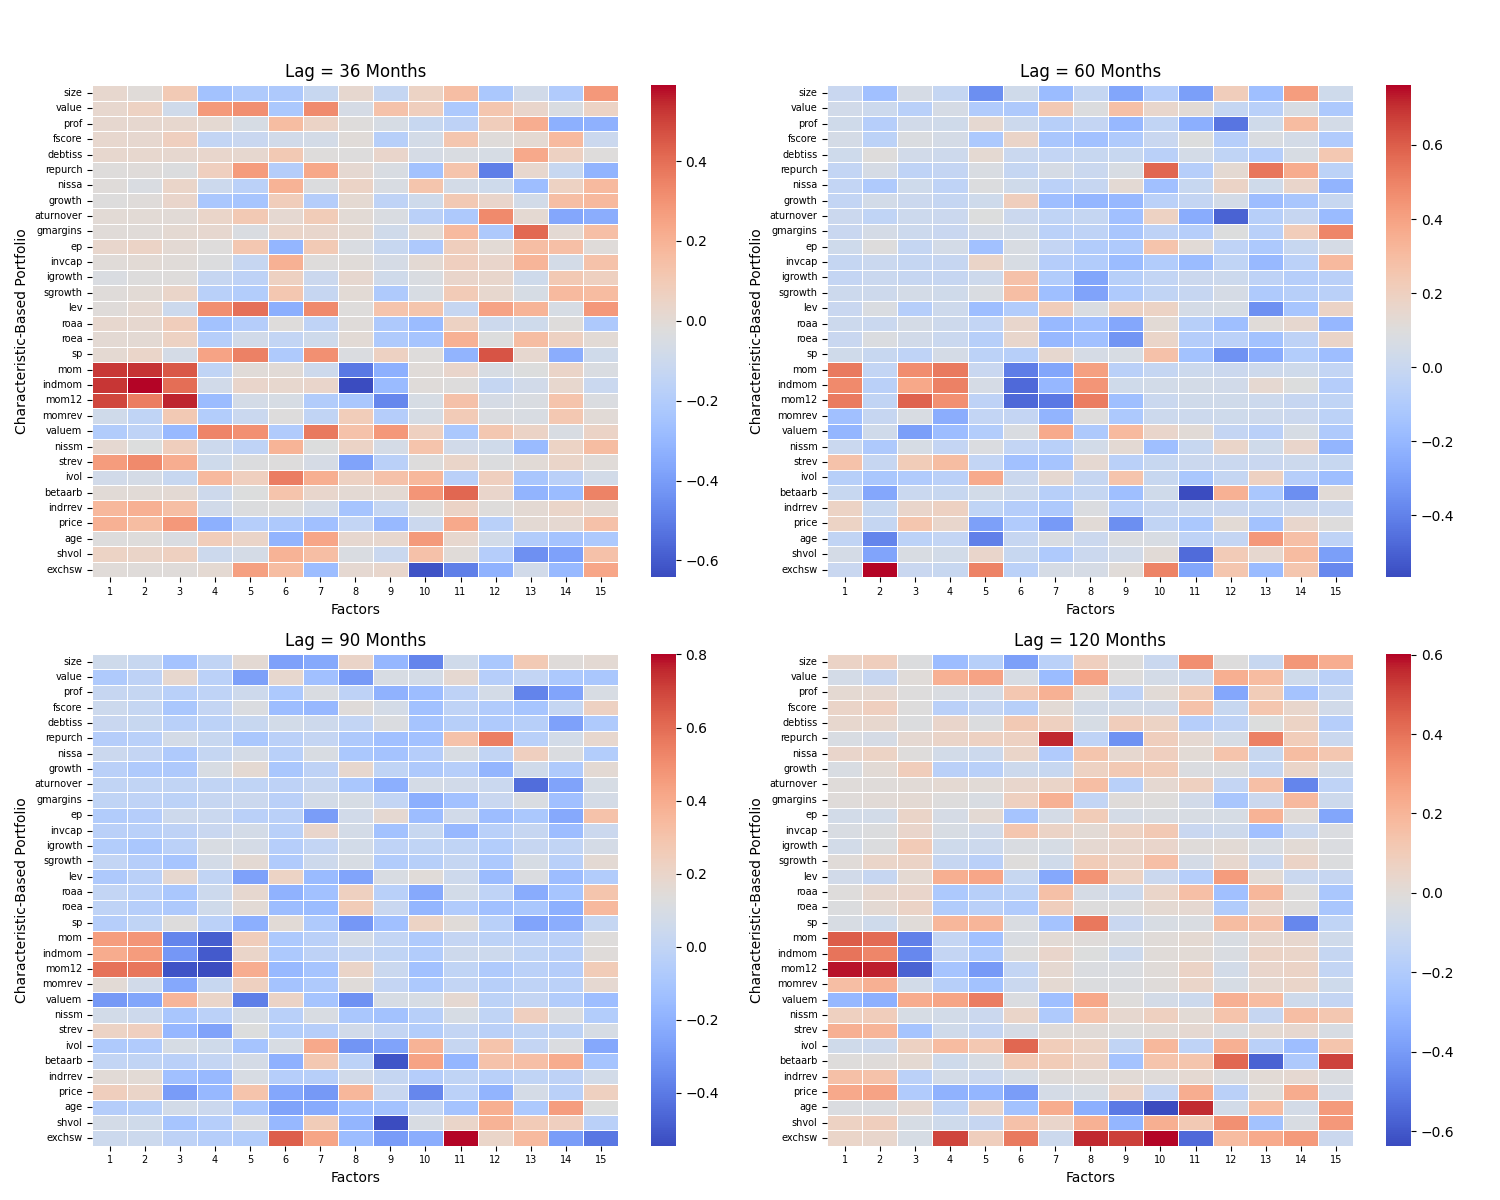
\includegraphics[width=0.85\linewidth]{B_15.png}
    \caption{Cross-Sectional Loadings, K = 15}
    \label{fig:B_15}
\end{figure}
\begin{figure}[H]
    \centering
    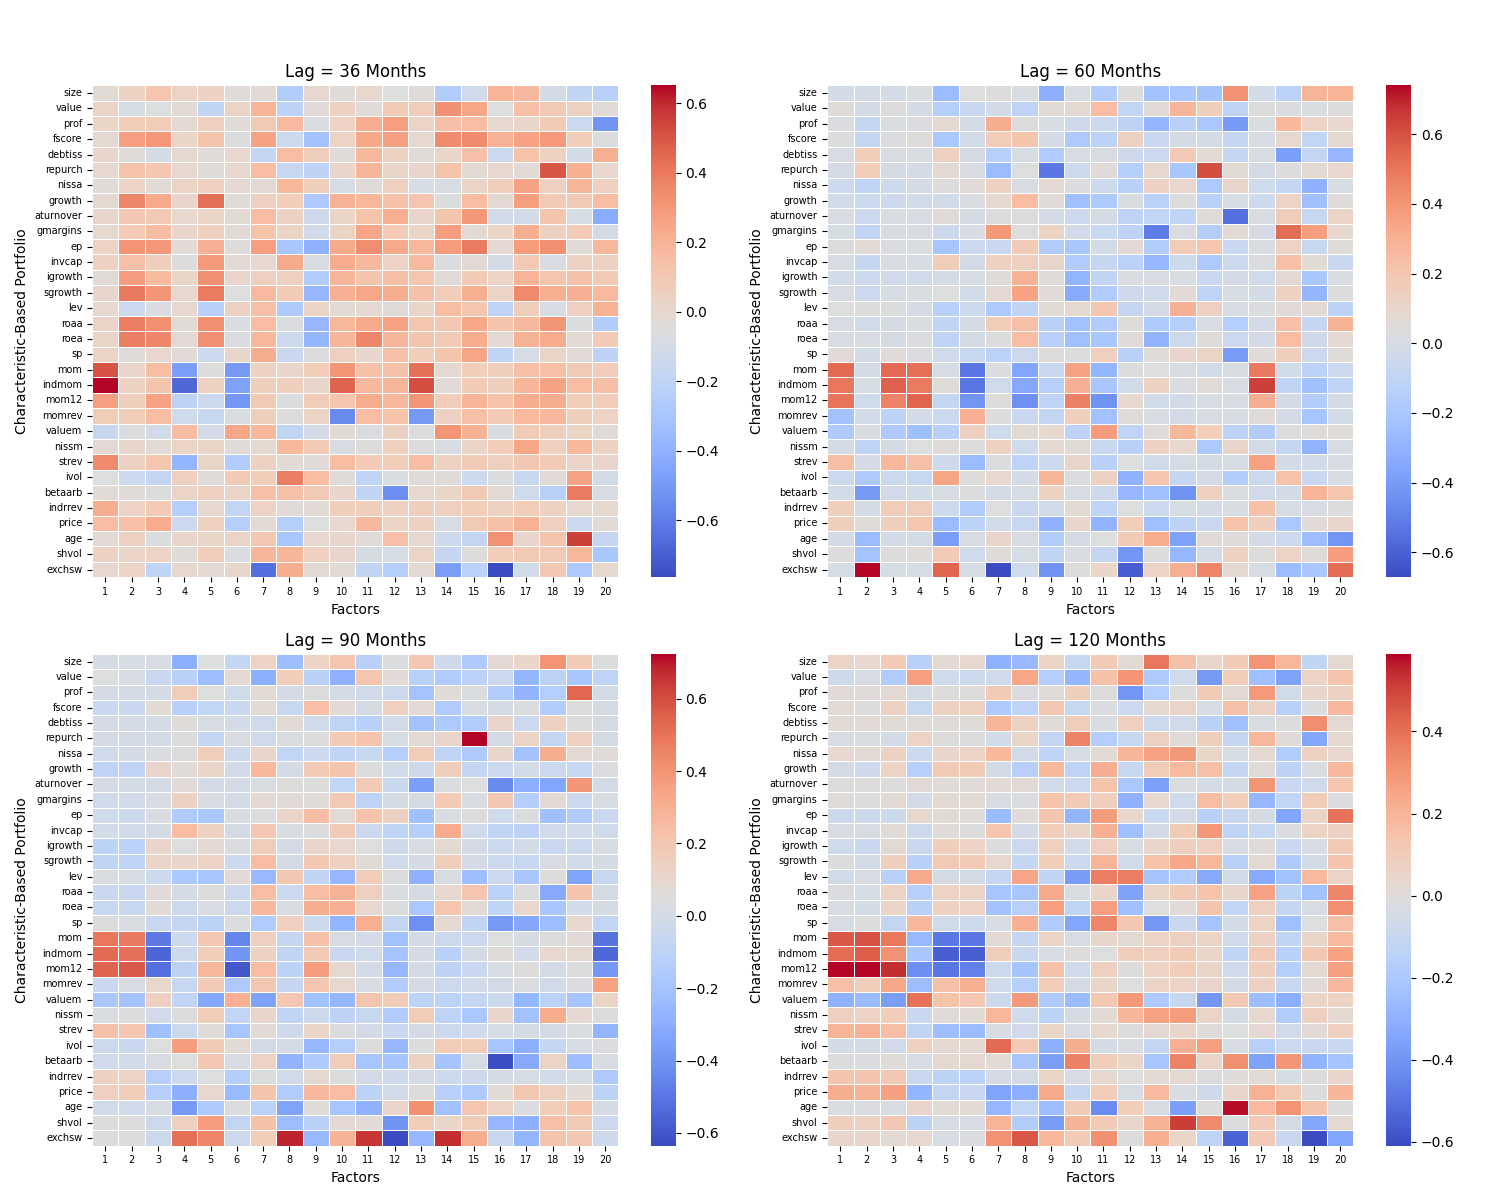
\includegraphics[width=0.85\linewidth]{B_20.png}
    \caption{Cross-Sectional Loadings, K = 20}
    \label{fig:B_20}
\end{figure}

\subsubsection{Lag Loadings / Decay Weights}

The decay weights (ie. lag loadings) are of primary interest to us because they shed light on the anomaly decay 
for different characteristic-sorted portfolios.

\begin{figure}[H]
    \centering
    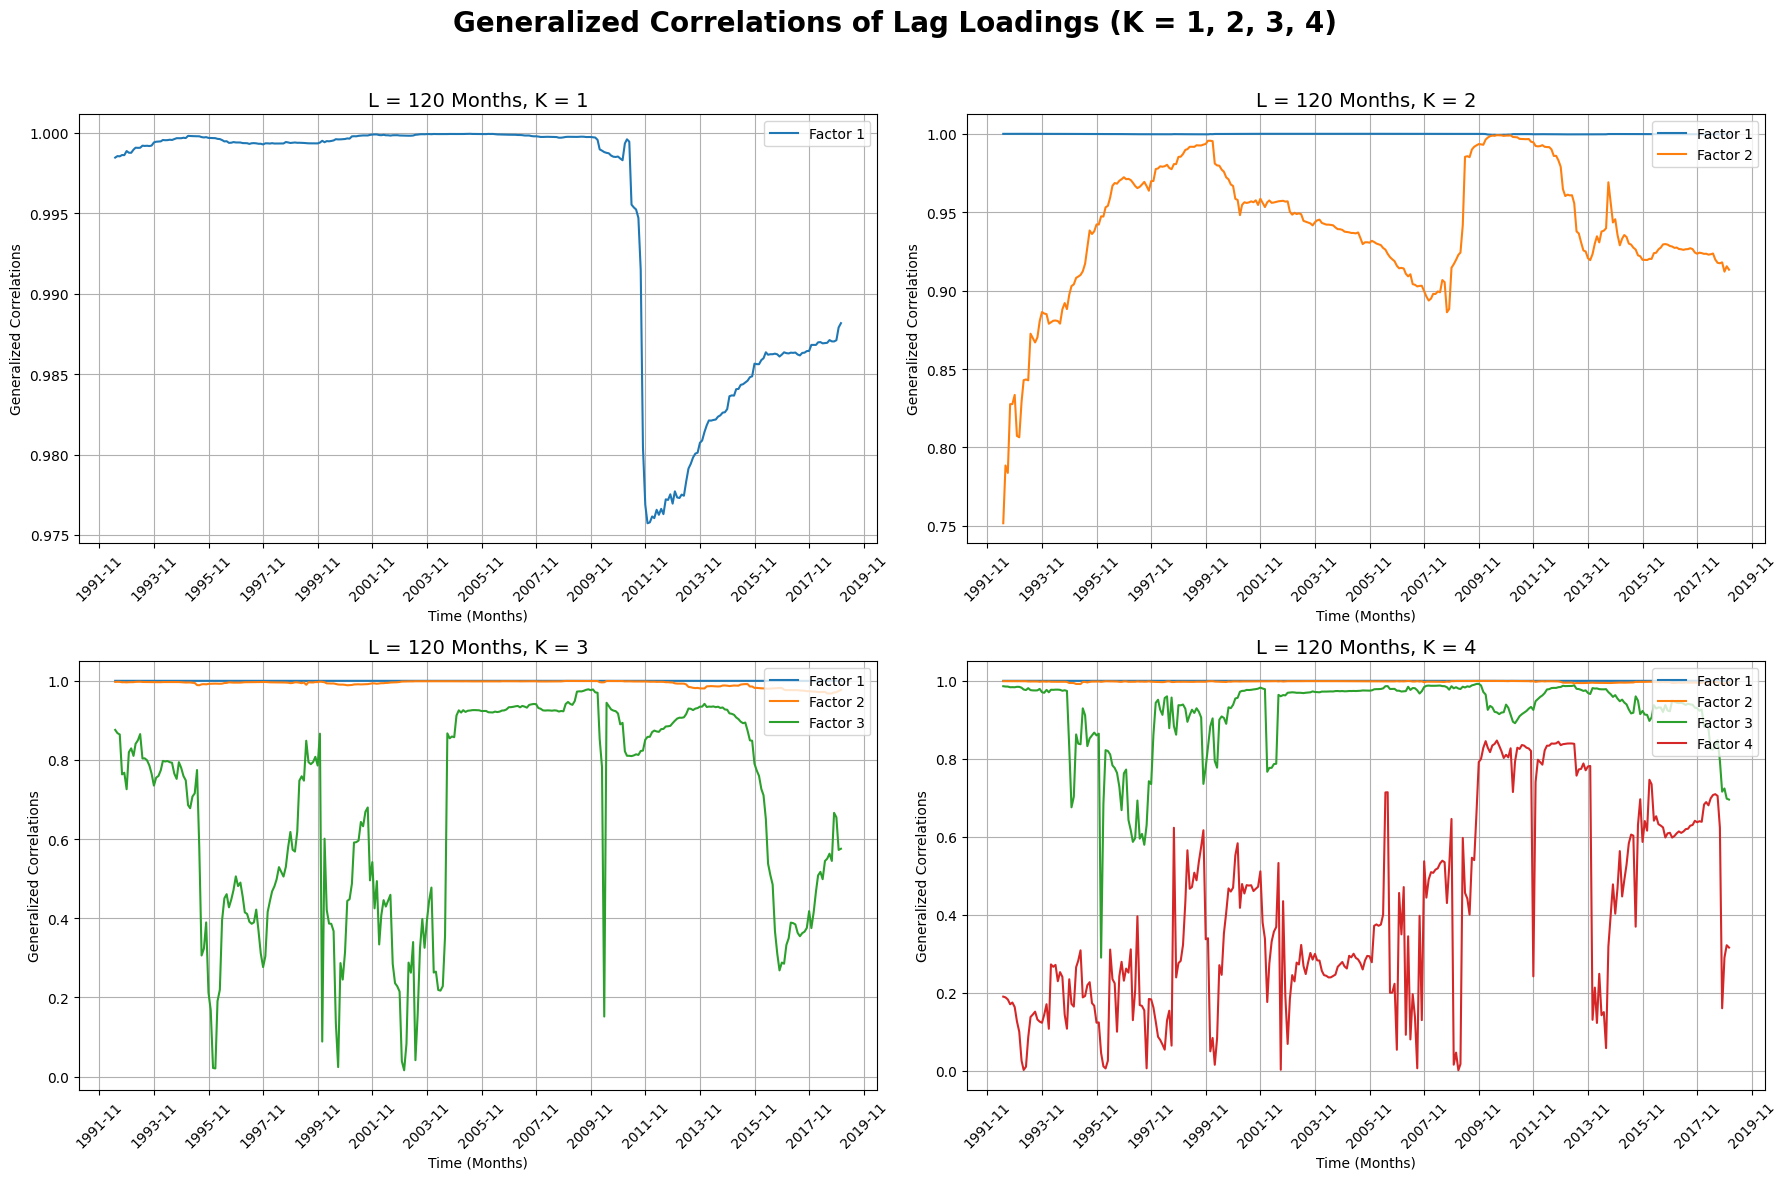
\includegraphics[width=0.85\linewidth]{W_gc_1.png}
    \caption{Generalized Correlations, K = 1, 2, 3, 4, Lag = 36 Months}
    \label{fig:W_gc_1}
\end{figure}
\begin{figure}[H]
    \centering
    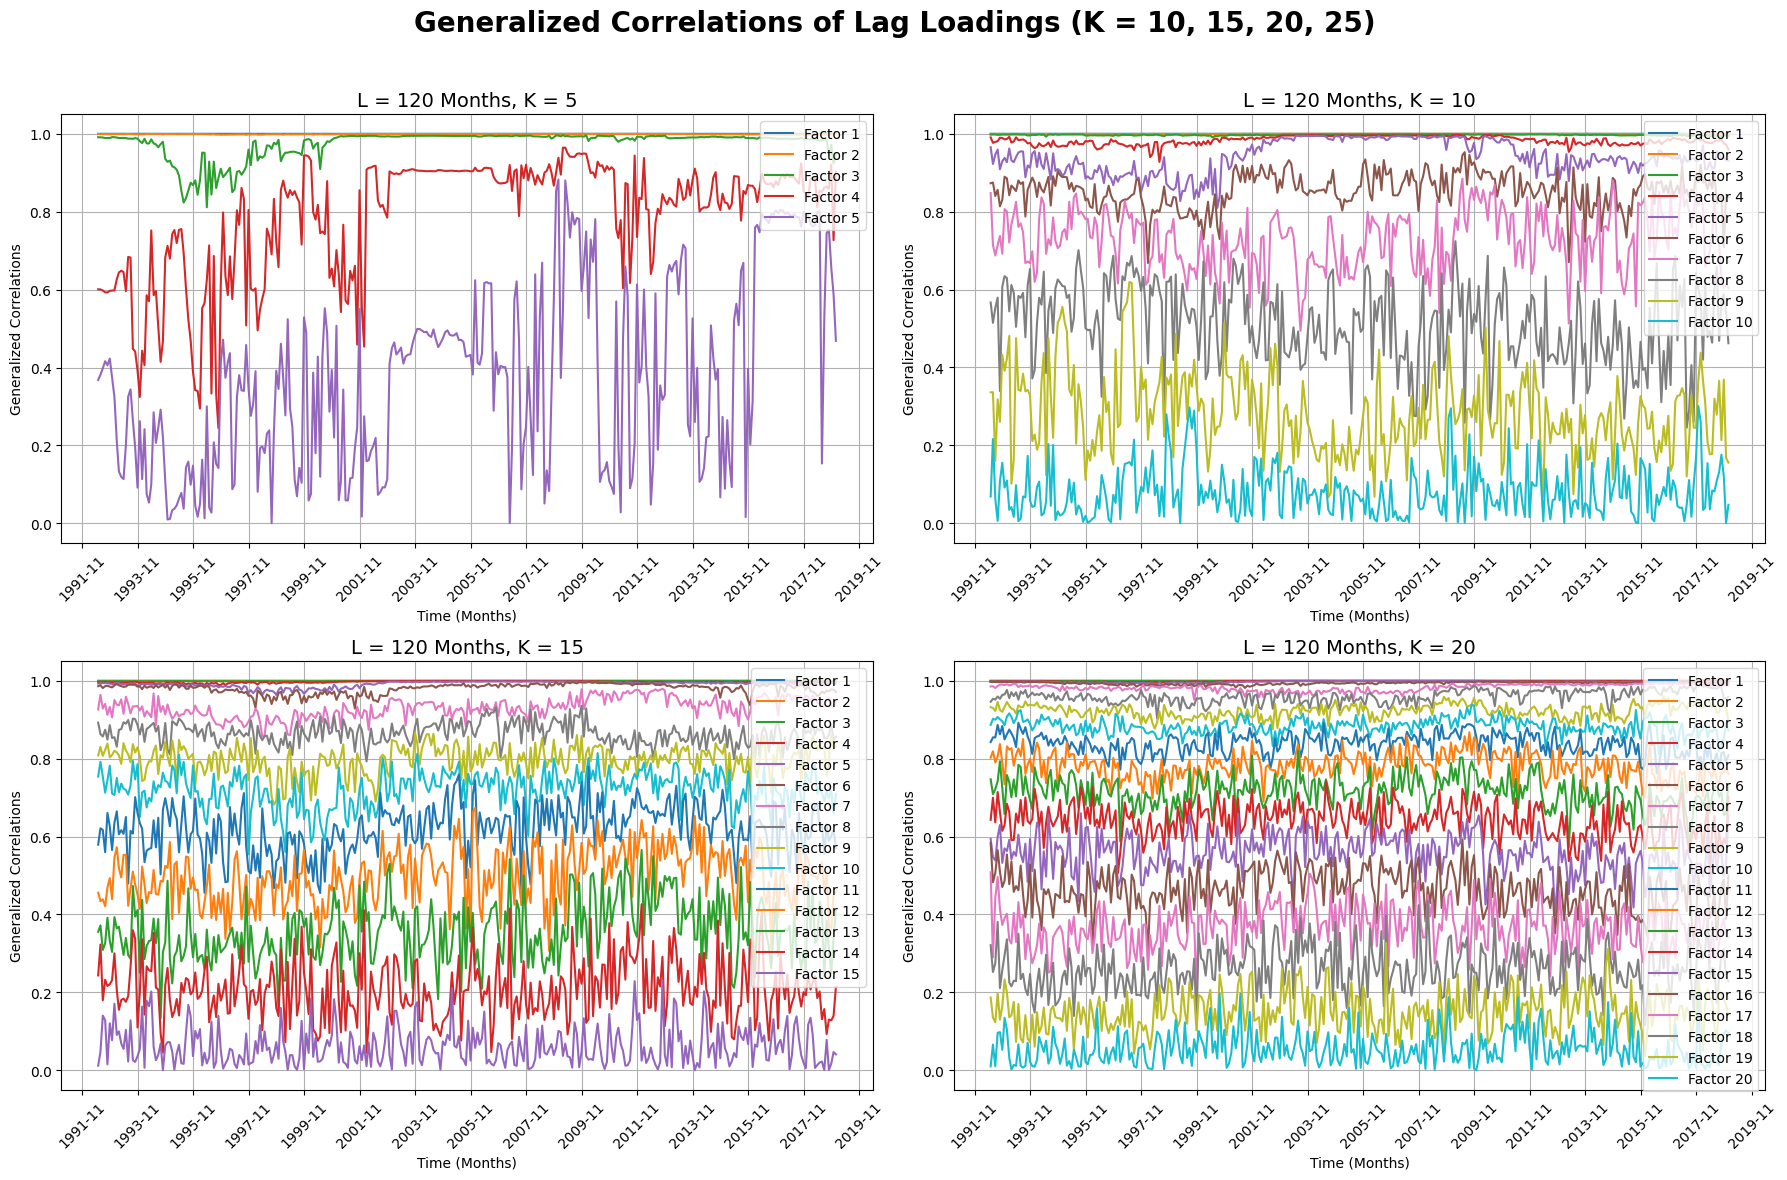
\includegraphics[width=0.85\linewidth]{W_gc_2.png}
    \caption{Generalized Correlations, K = 5, 10, 15, 20, Lag = 36 Months}
    \label{fig:W_gc_2}
\end{figure}

Dates on the x-axis are trading days ie. the local model uses a $120$-month rolling window that 
ends on that date. In most plots, $\approx \frac{1}{2}$ of the factors' lag loadings are at least 
$90\%$ correlated with the global estimate throughout the entire duration. 

\begin{figure}[H]
    \centering
    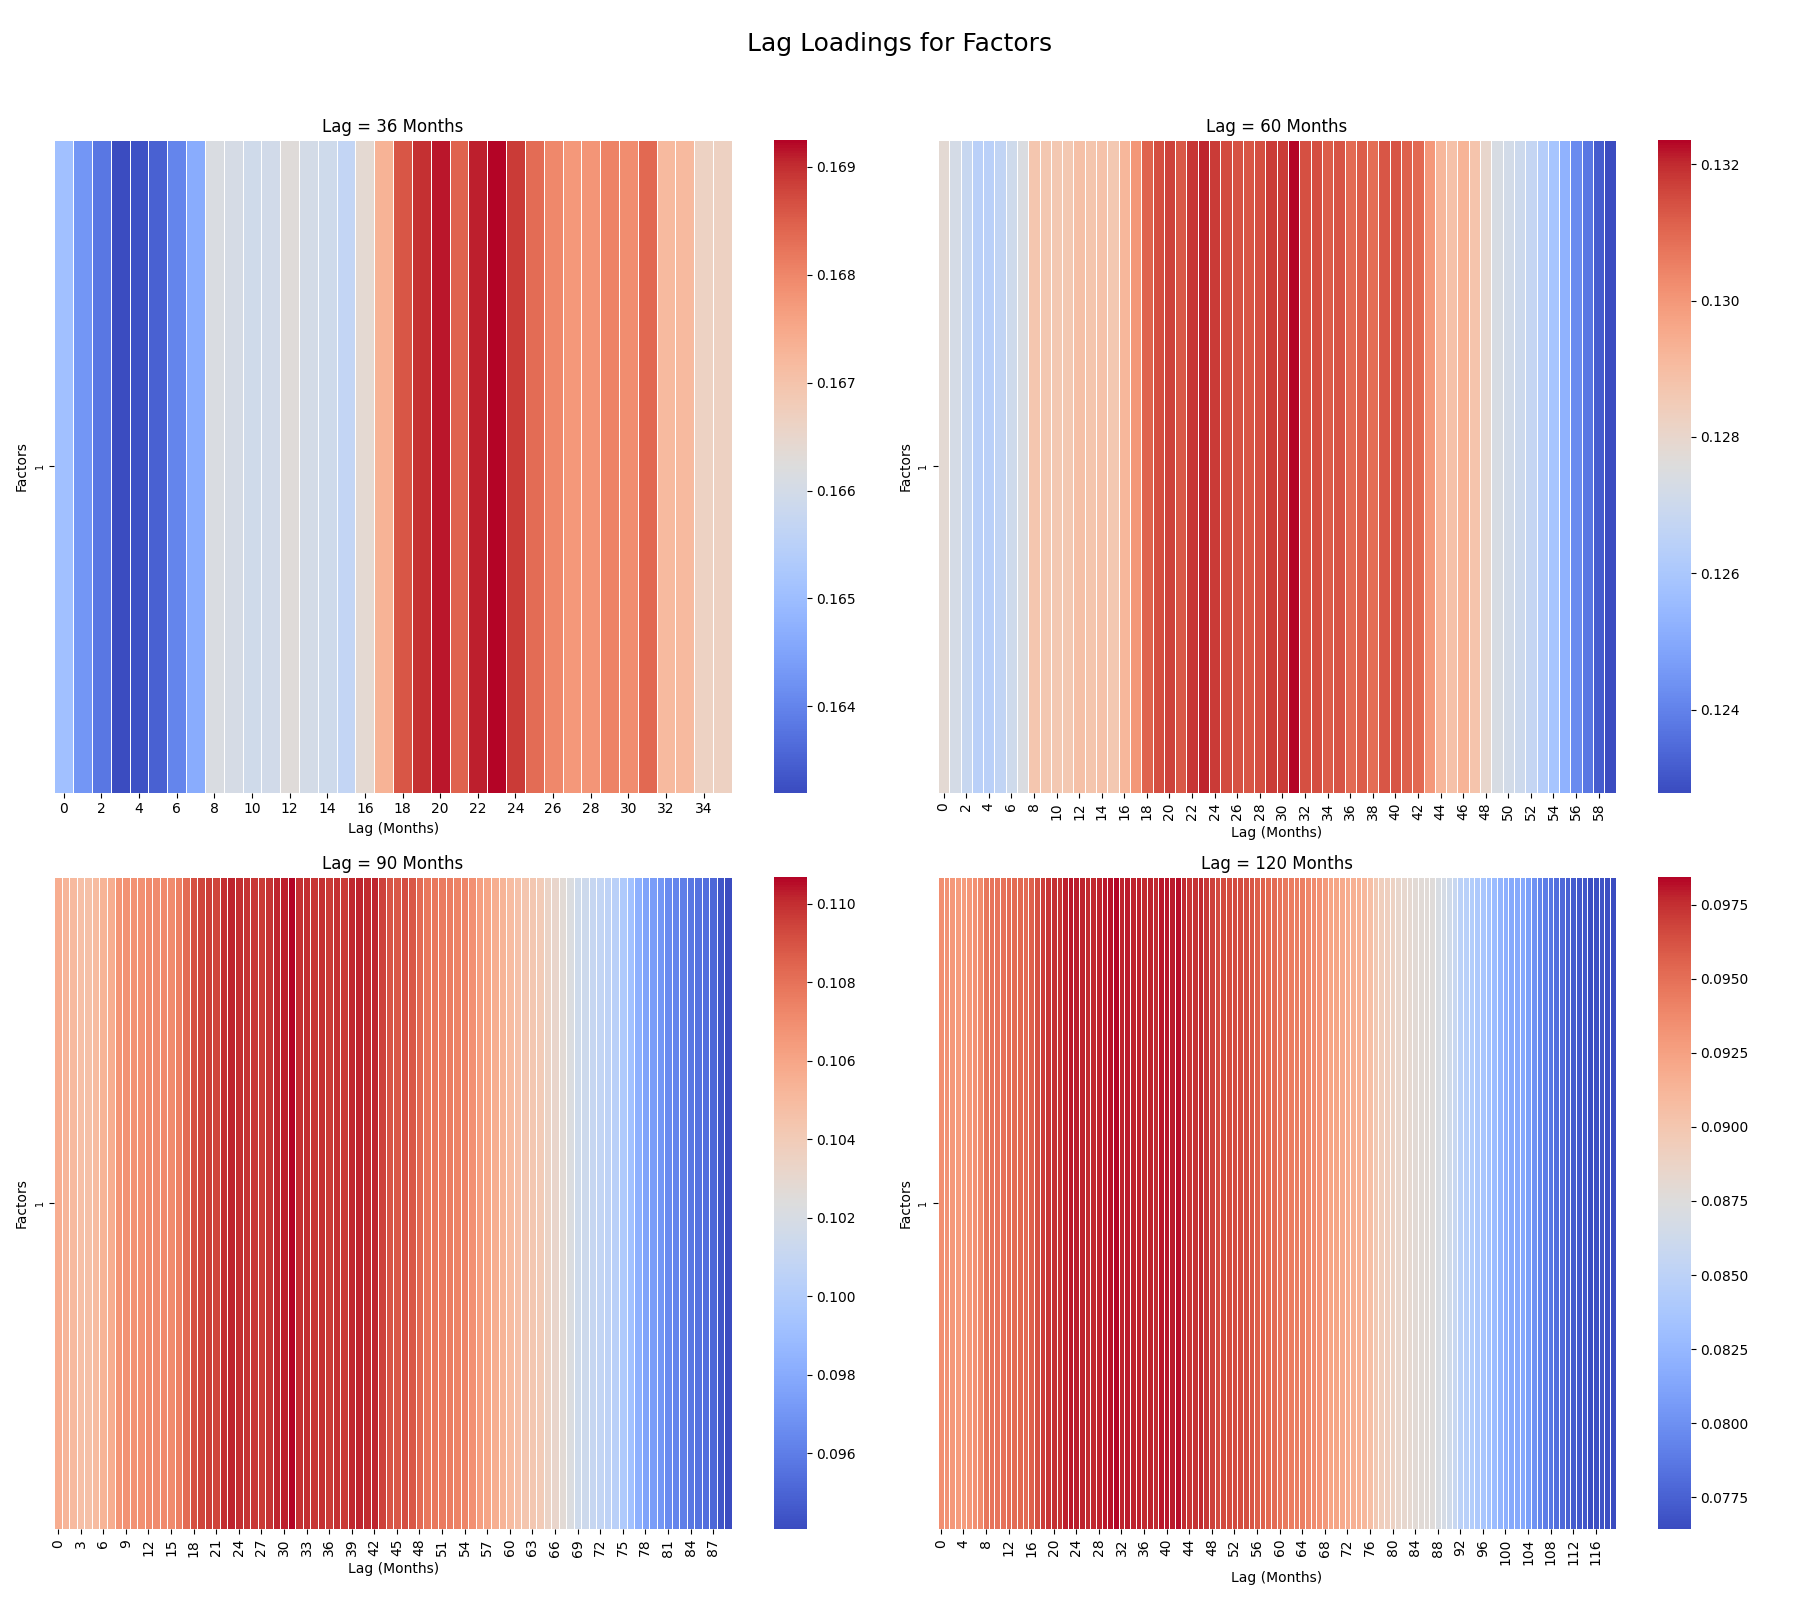
\includegraphics[width=0.85\linewidth]{W_1.png}
    \caption{Lag Loadings Heatmap, K = 1}
    \label{fig:W_1}
\end{figure}
\begin{figure}[H]
    \centering
    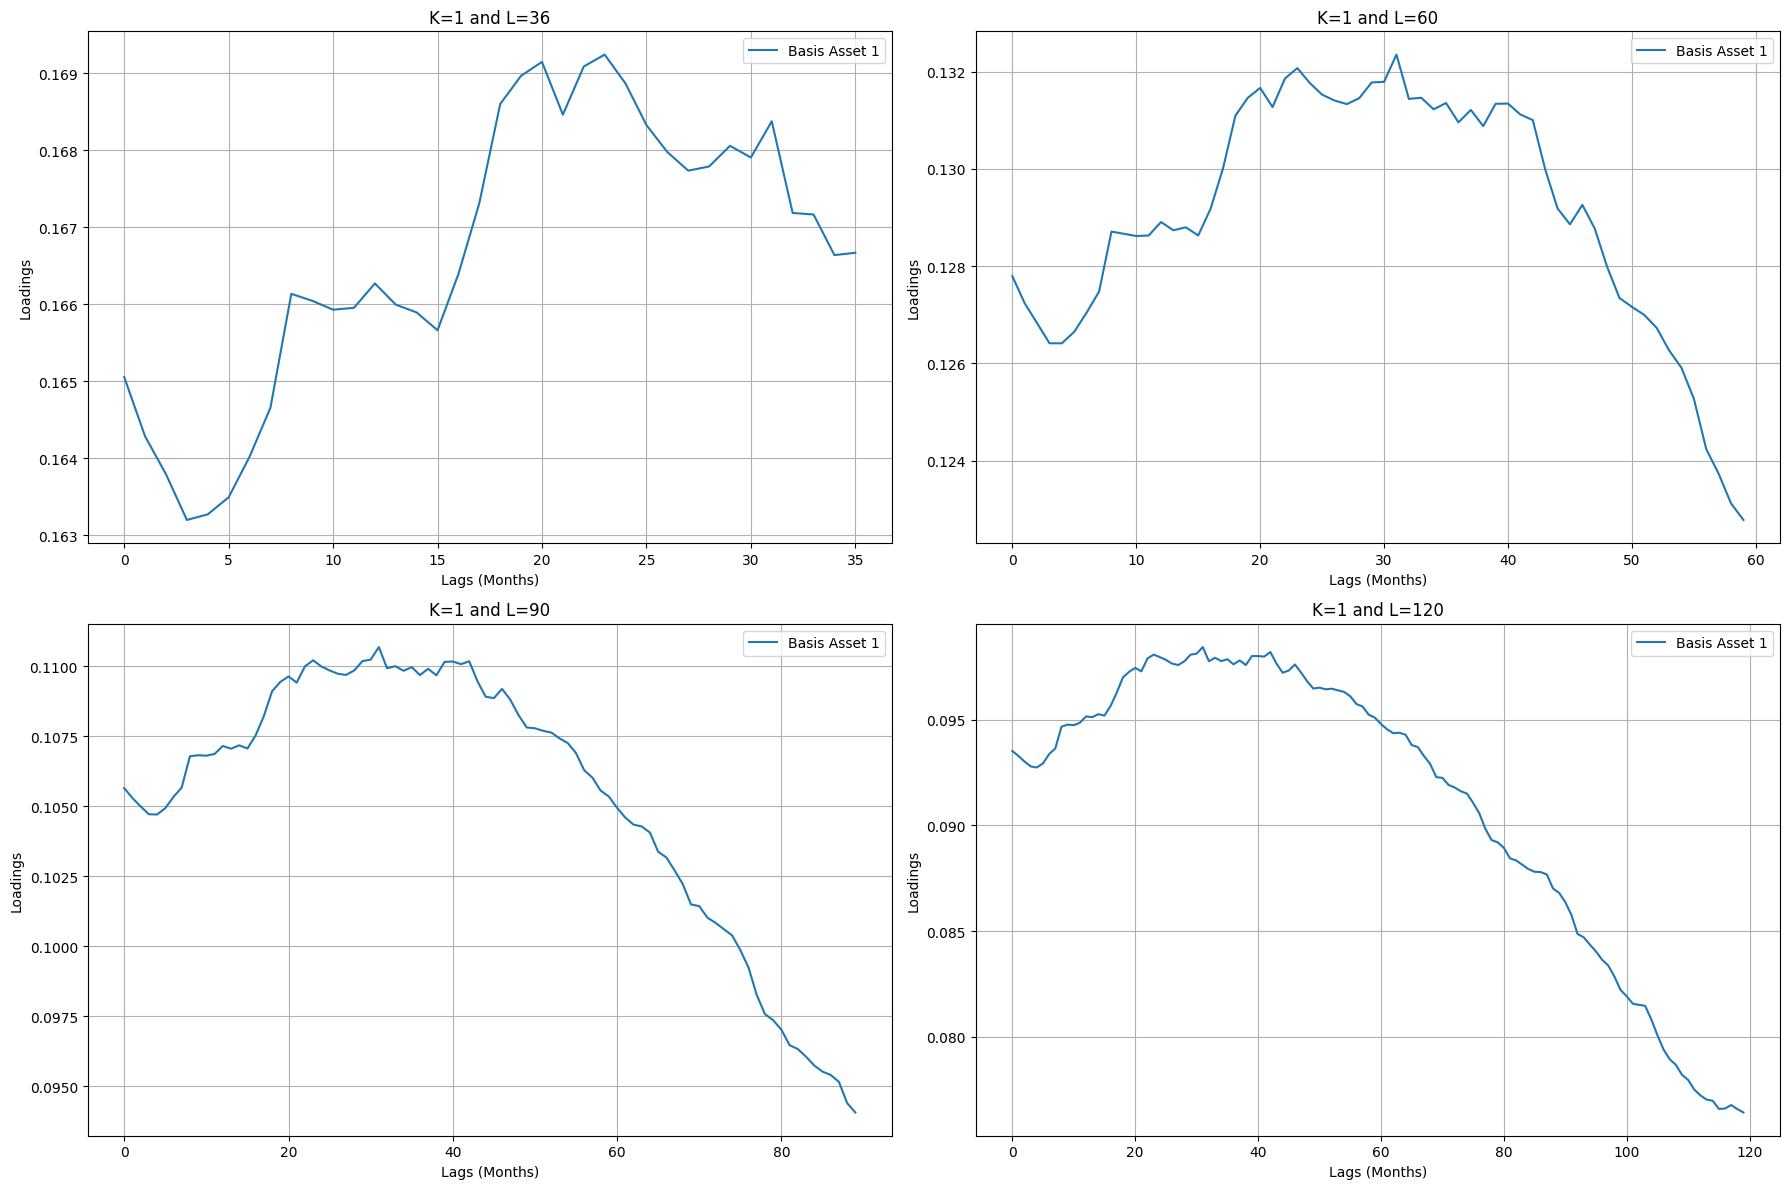
\includegraphics[width=0.85\linewidth]{W_1_line.png}
    \caption{Lag Loadings Line Plot, K = 1}
    \label{fig:W_1_line}
\end{figure}
\begin{figure}[H]
    \centering
    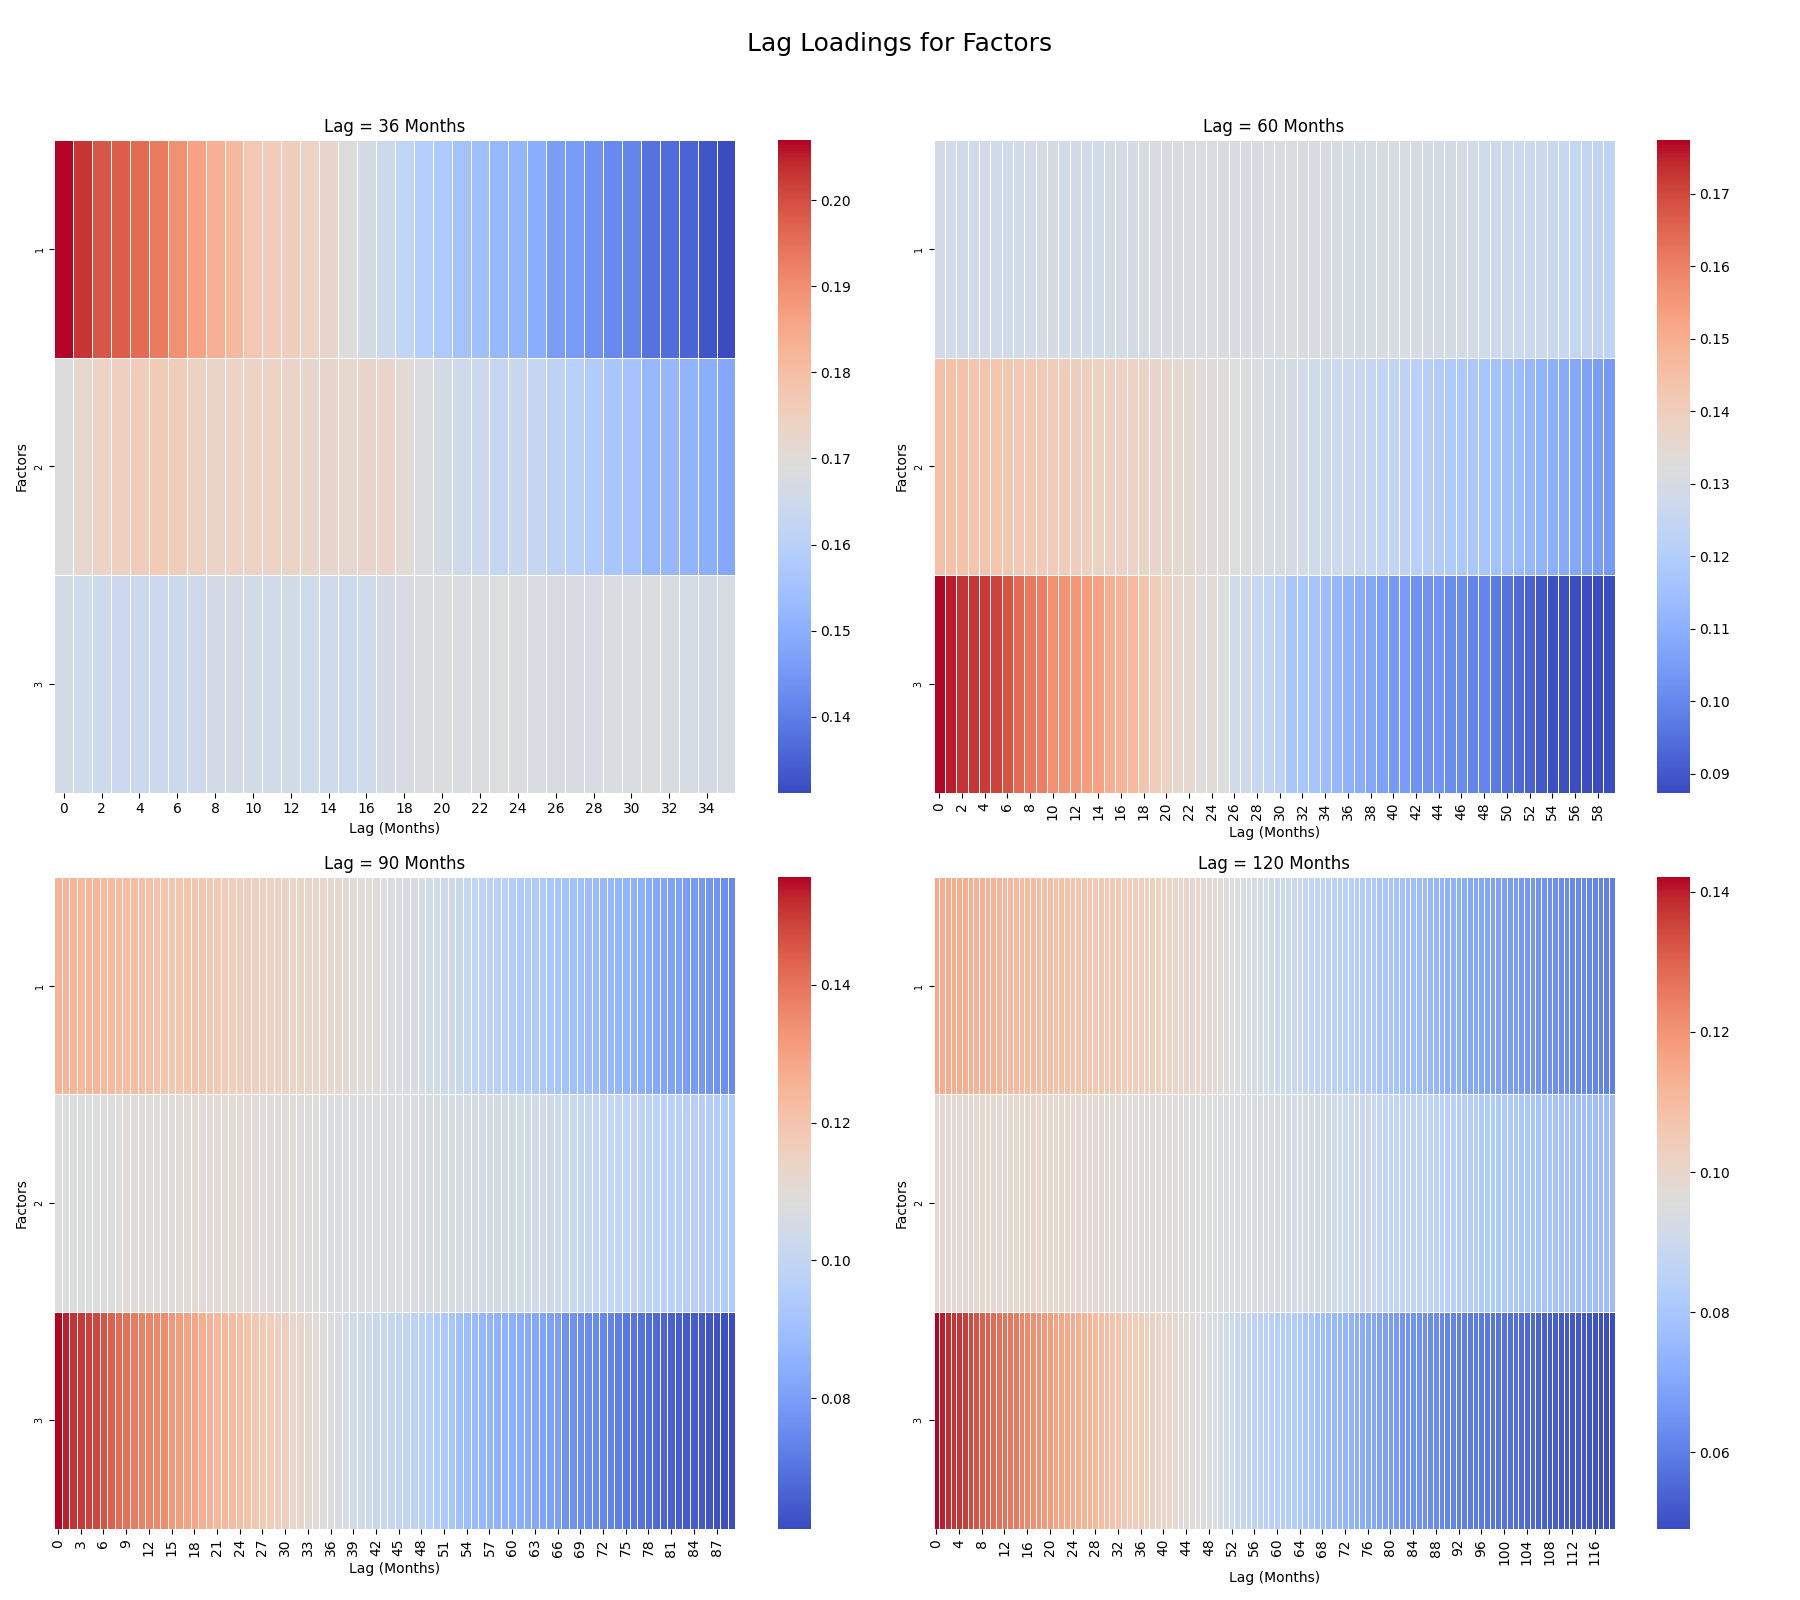
\includegraphics[width=0.85\linewidth]{W_3.png}
    \caption{Lag Loadings Heatmap, K = 3}
    \label{fig:W_3}
\end{figure}
\begin{figure}[H]
    \centering
    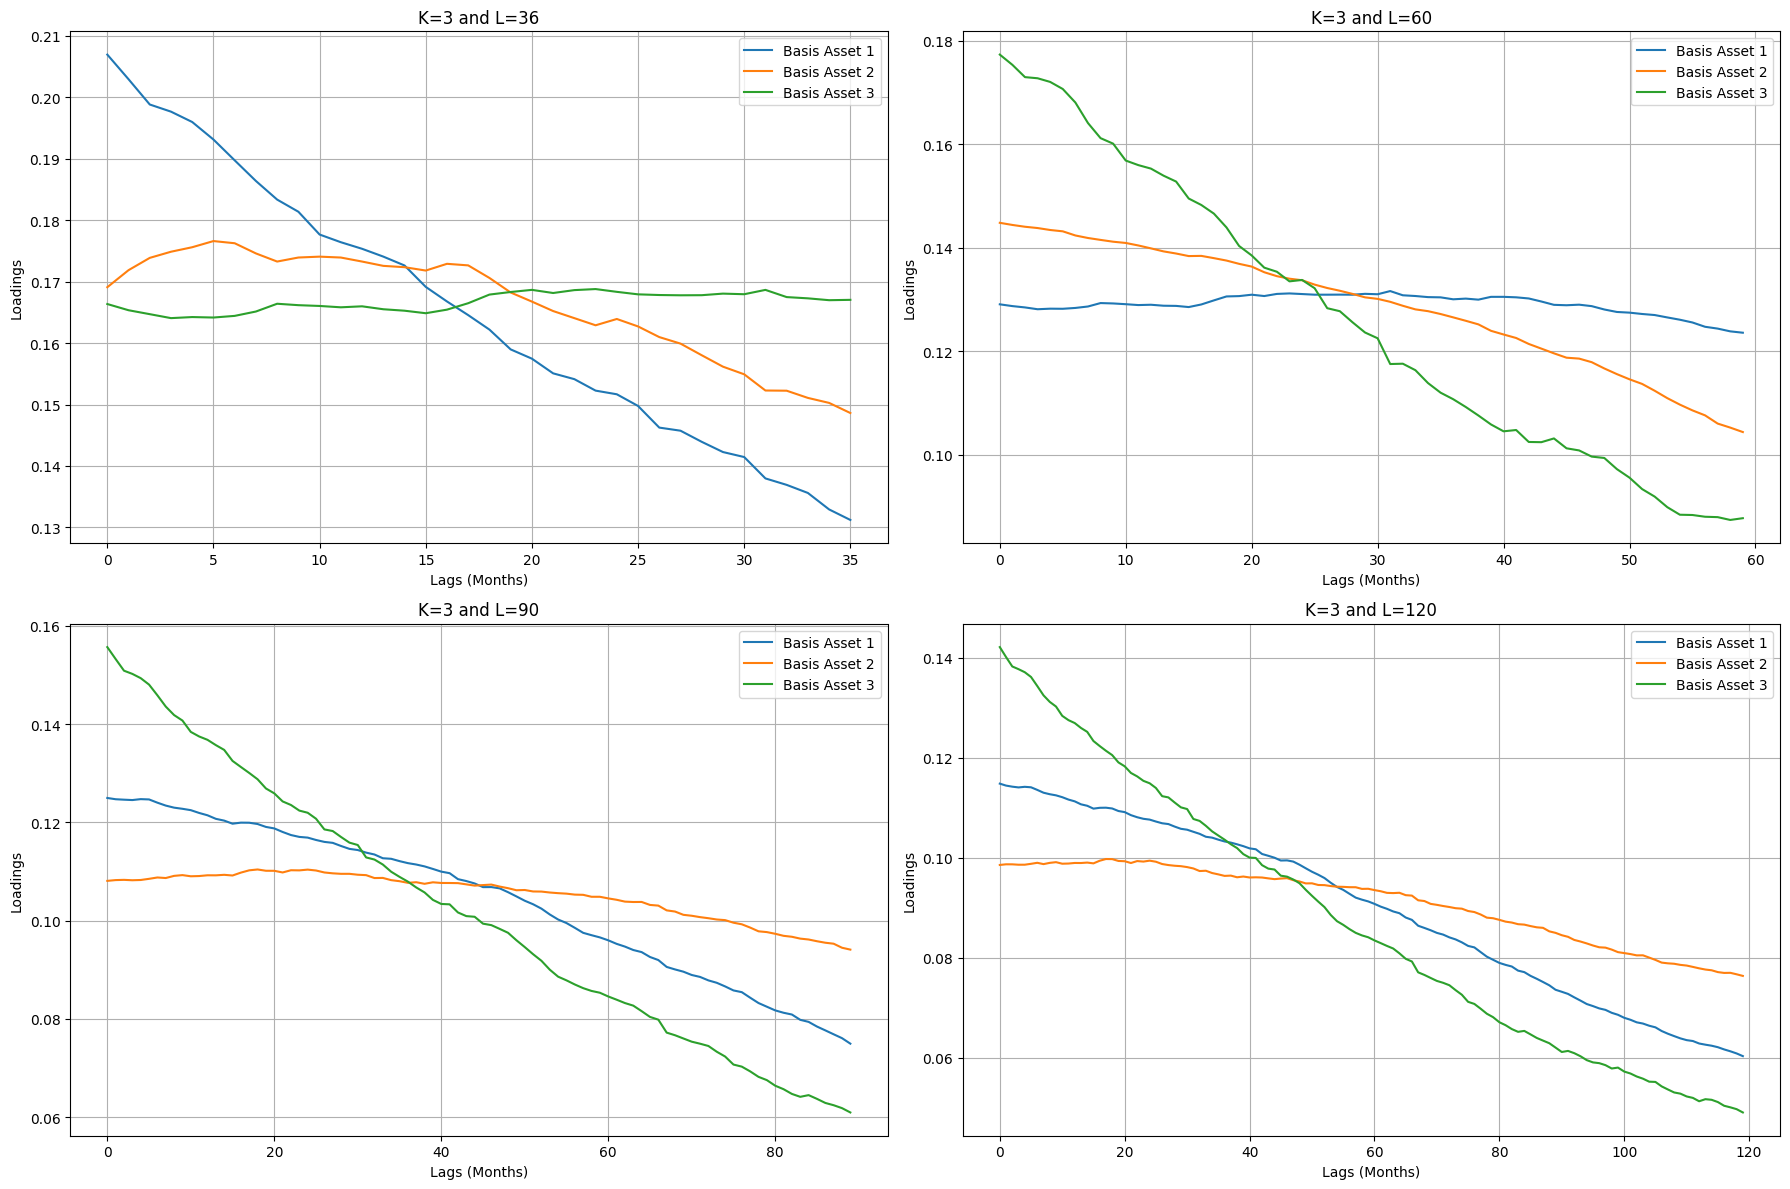
\includegraphics[width=0.85\linewidth]{W_3_line.png}
    \caption{Lag Loadings Line Plot, K = 3}
    \label{fig:W_3_line}
\end{figure}

\begin{figure}[H]
    \centering
    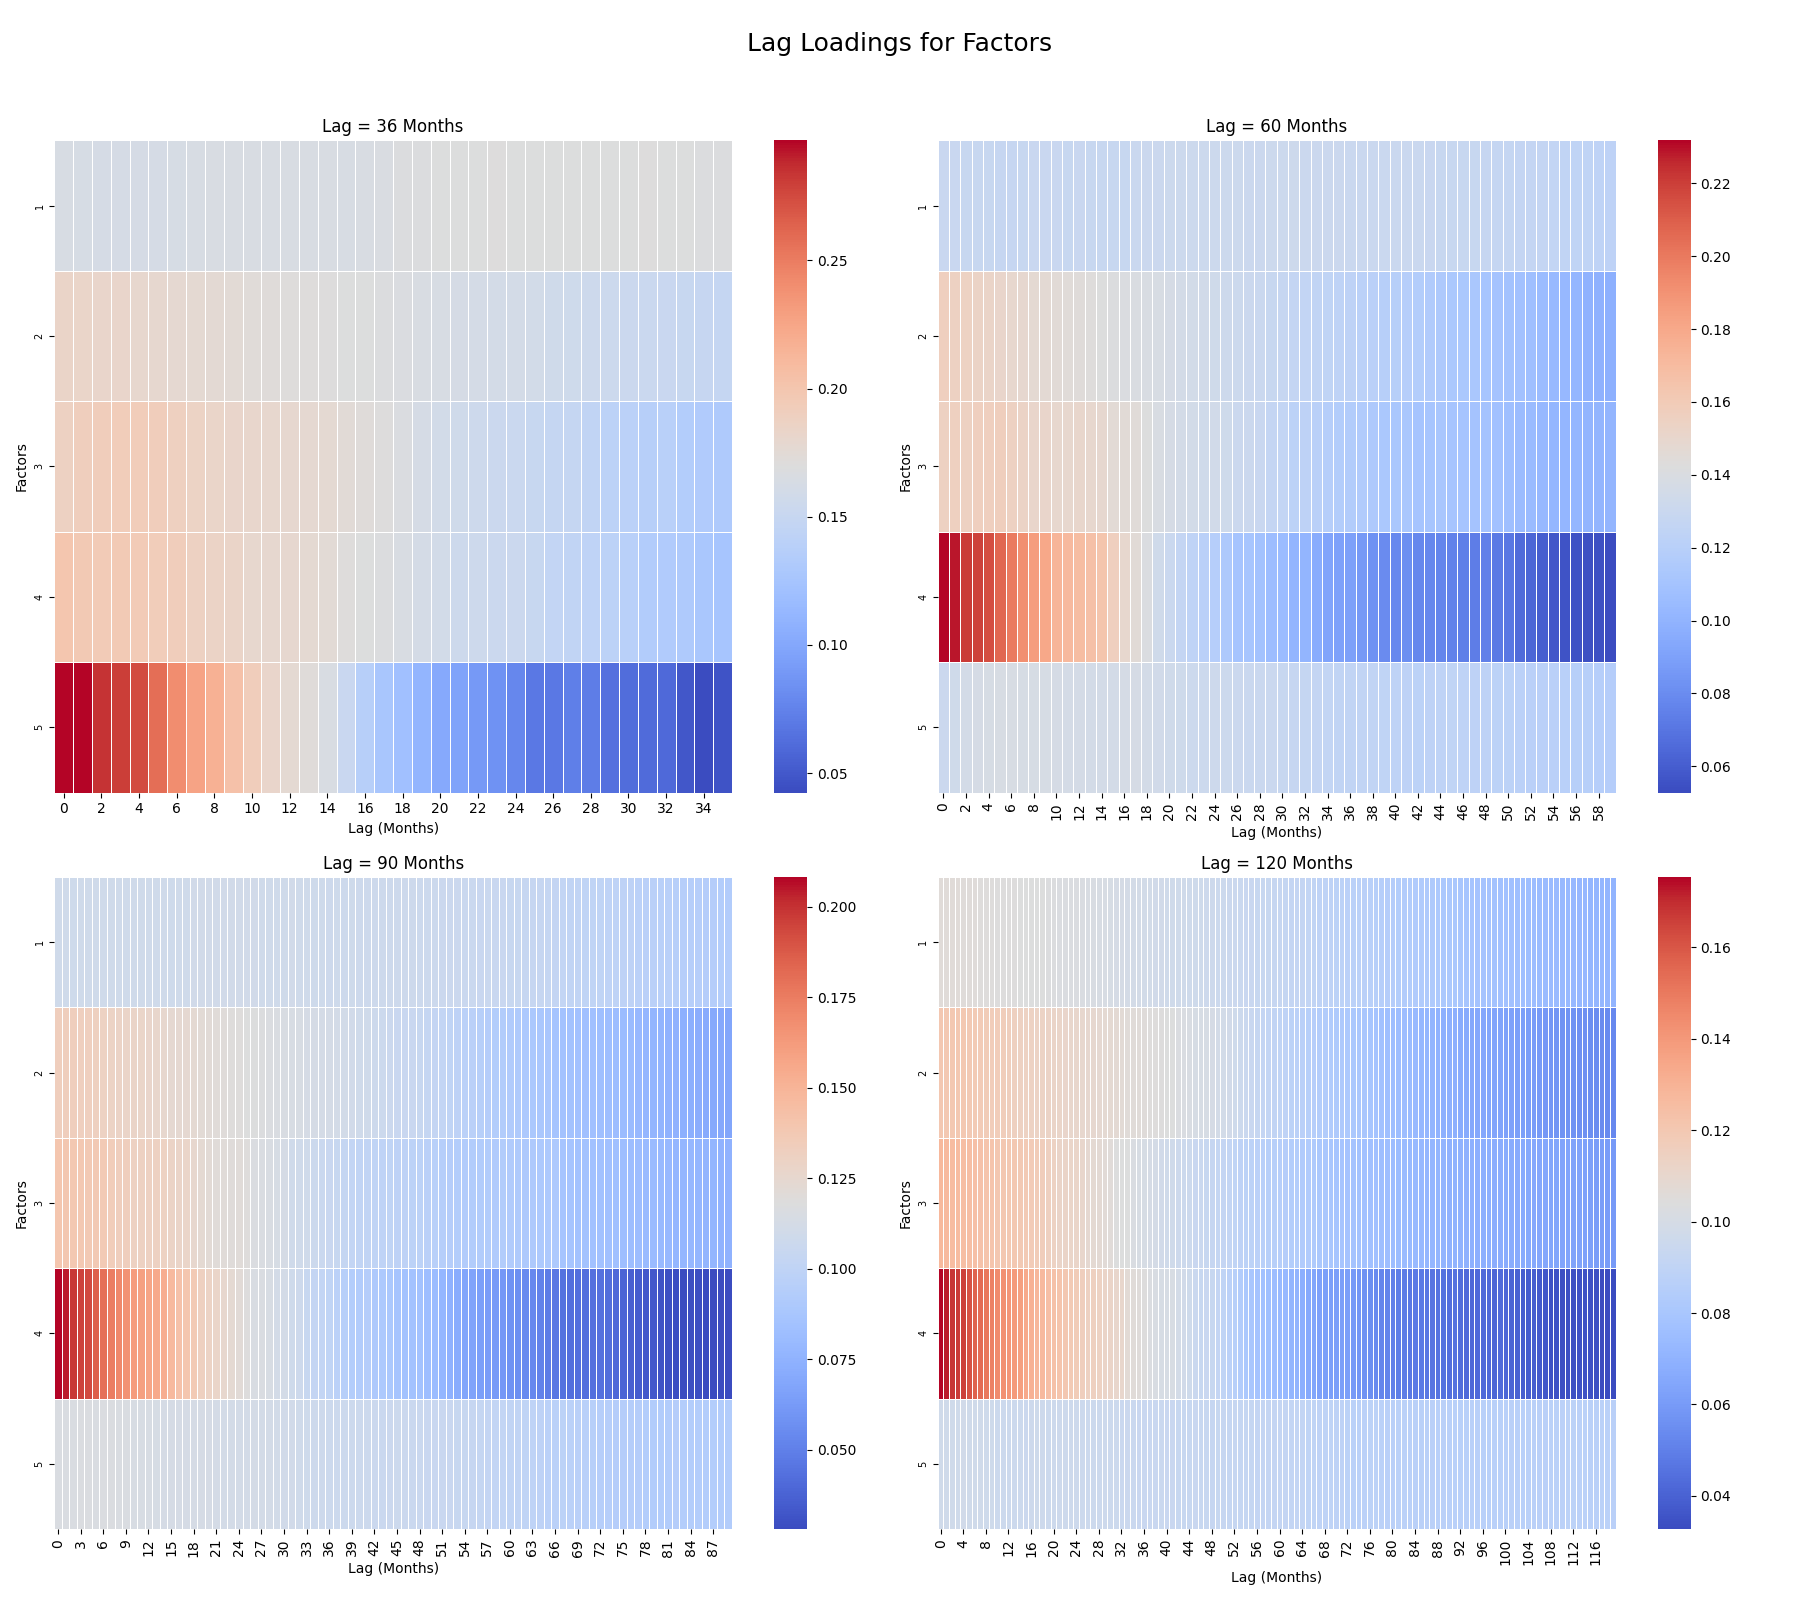
\includegraphics[width=0.85\linewidth]{W_5.png}
    \caption{Lag Loadings Heatmap, K = 5}
    \label{fig:W_5}
\end{figure}
\begin{figure}[H]
    \centering
    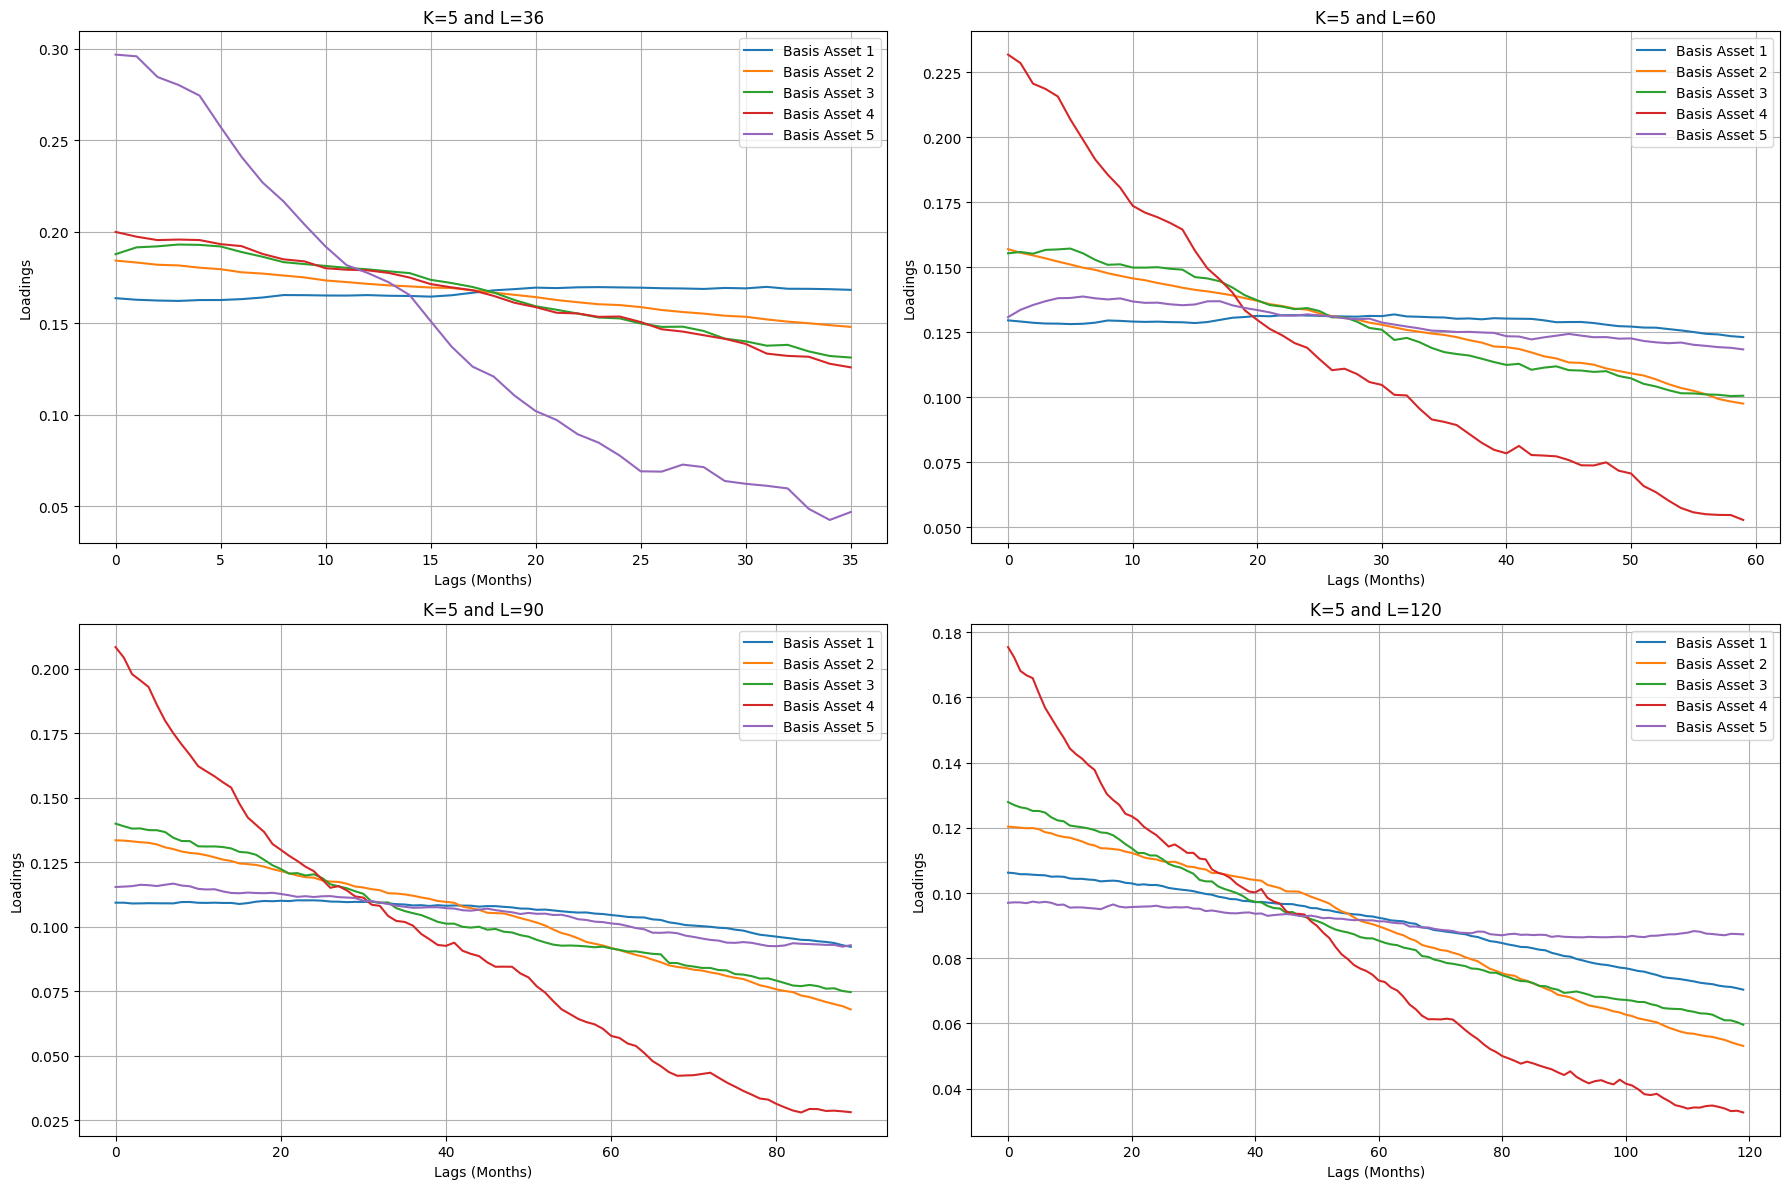
\includegraphics[width=0.85\linewidth]{W_5_line.png}
    \caption{Lag Loadings Line Plot, K = 5}
    \label{fig:W_5_line}
\end{figure}

\begin{figure}[H]
    \centering
    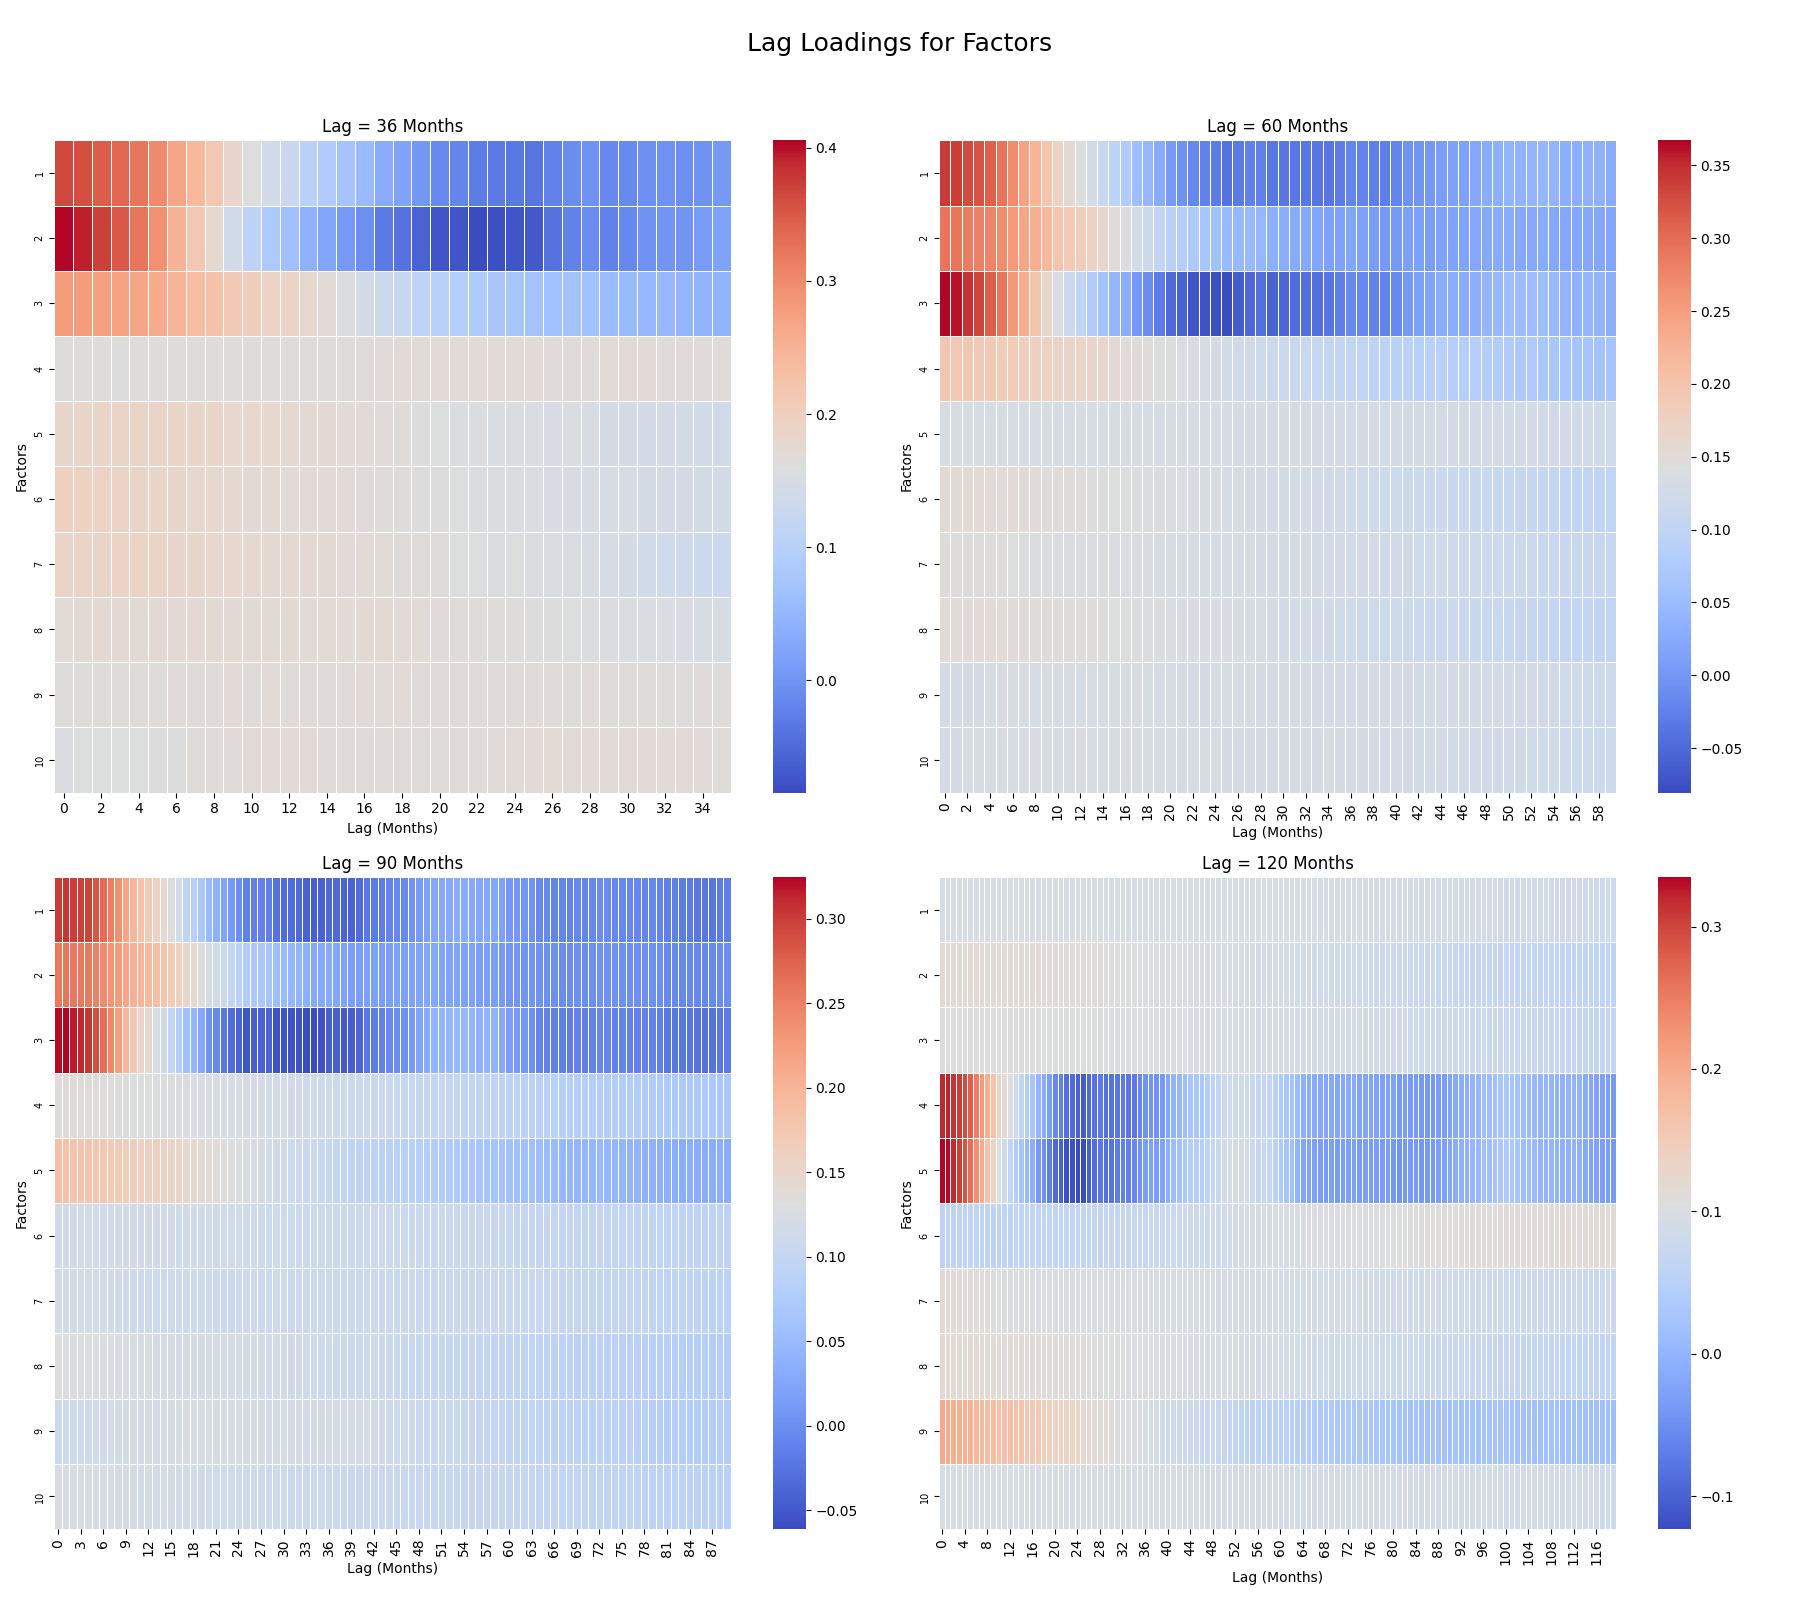
\includegraphics[width=0.85\linewidth]{W_10.png}
    \caption{Lag Loadings Heatmap, K = 10}
    \label{fig:W_10}
\end{figure}
\begin{figure}[H]
    \centering
    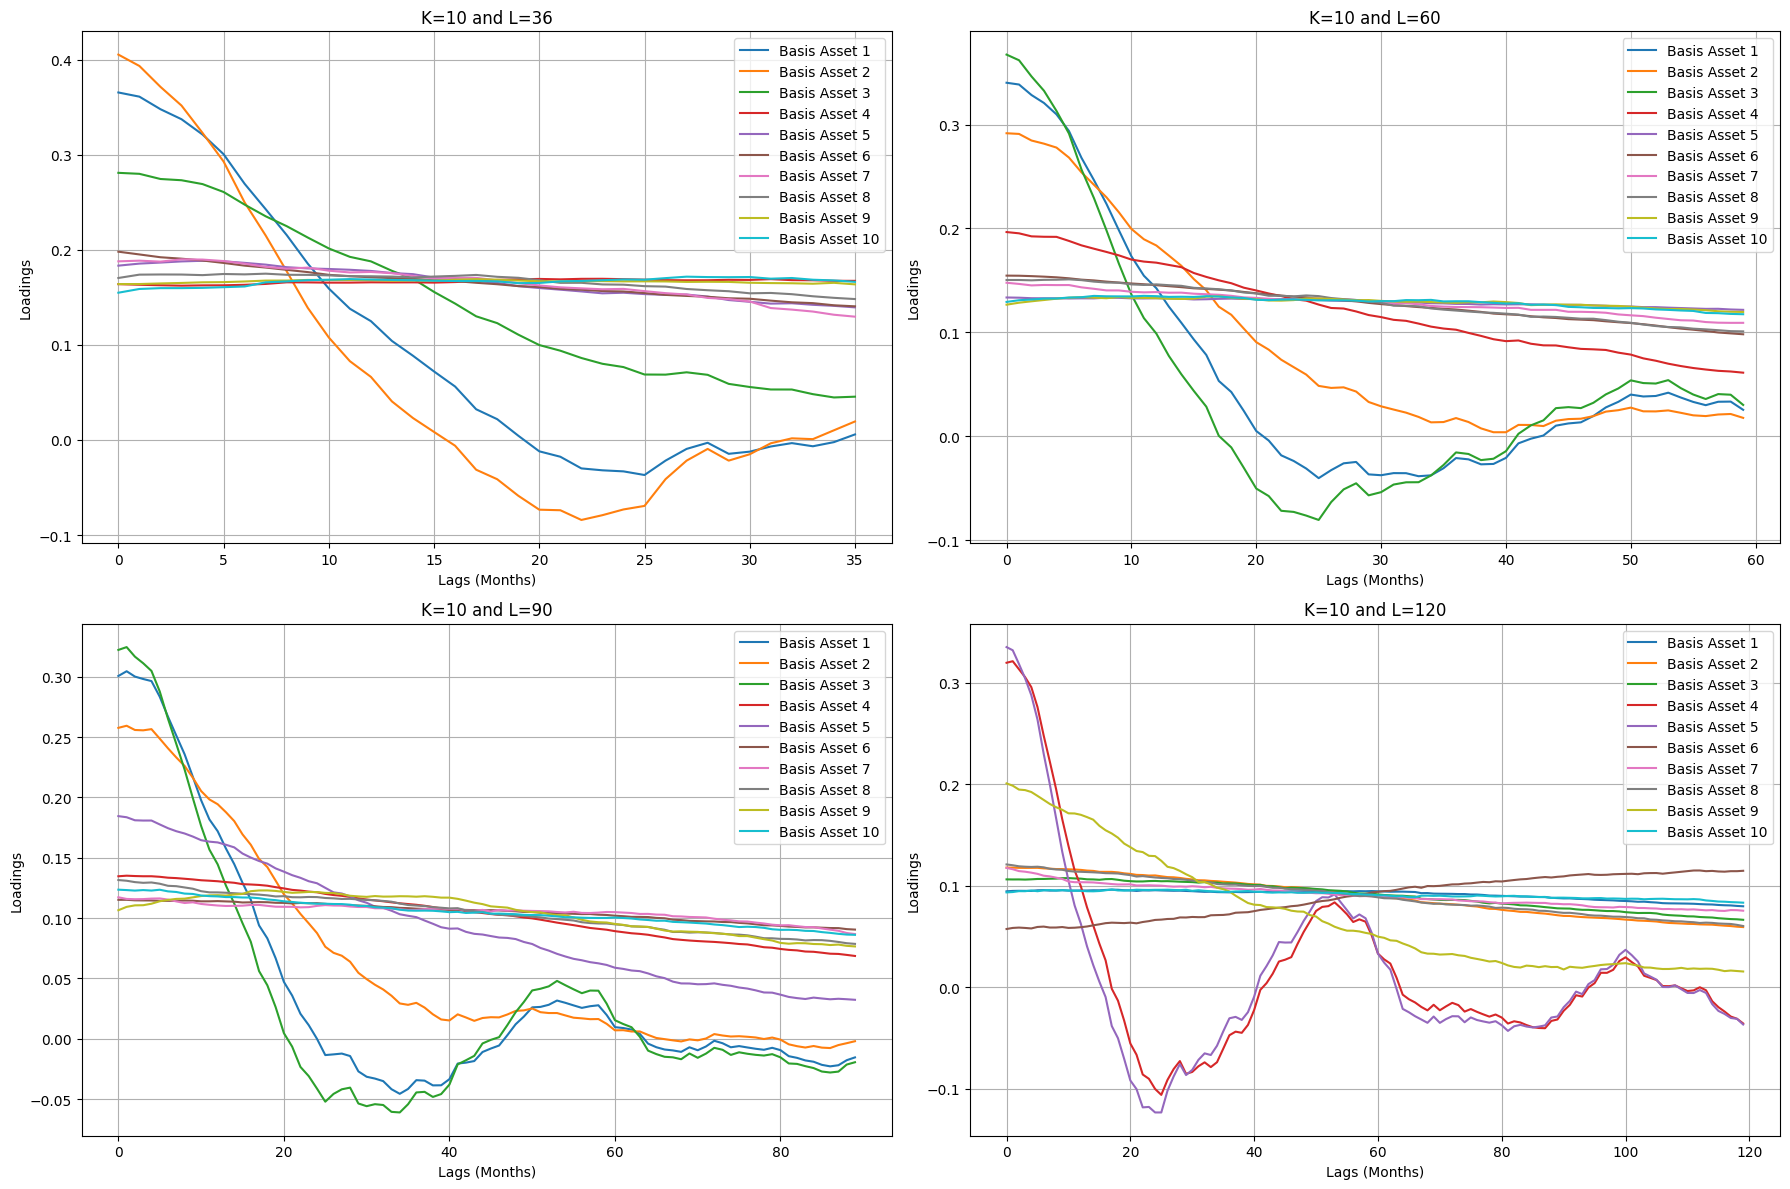
\includegraphics[width=0.85\linewidth]{W_10_line.png}
    \caption{Lag Loadings Line Plot, K = 10}
    \label{fig:W_10_line}
\end{figure}


We could look at things like generalized correlations, line plots of the lag loadings, but it's ultimately 
difficult to extract anything meaningful from this without understanding how the latent factors load 
on the original portfolios. We have this transformation via the $\bm{B}$ matrix. 

\subsubsection{Lag Loadings In Terms of Characteristic-Based Portfolios}


\begin{itemize}
    \item We can also look at $\bm{W^B} \in \R^{N \times L}$, which explains how our original portfolios load on lags.
\end{itemize}
\begin{align}
    \bm{W^{B}} = \bm{B(B}^\top \bm{B)}^{-1} \bm{W}^\top
\end{align}
In this first set of plots, we estimate \bm{$W$} and \bm{$B$} in the full-sample where \bm{$B$} subsumes the scalar term, normalize them such that all 
basis assets have unit norm for the lag loadings, and then use the above formula $\bm{W^B}$. I denote these \emph{unnormalized} because 
each portfolio's loading on lags is not normalized, although $\bm{W}$ is. We can also normalize them to have unit norm; these 
norms can be subsumed by the scalar term. 

I think only magnitude of the weights decay matters, sign can be flipped or subsumed

\begin{figure}[H]
    \centering
    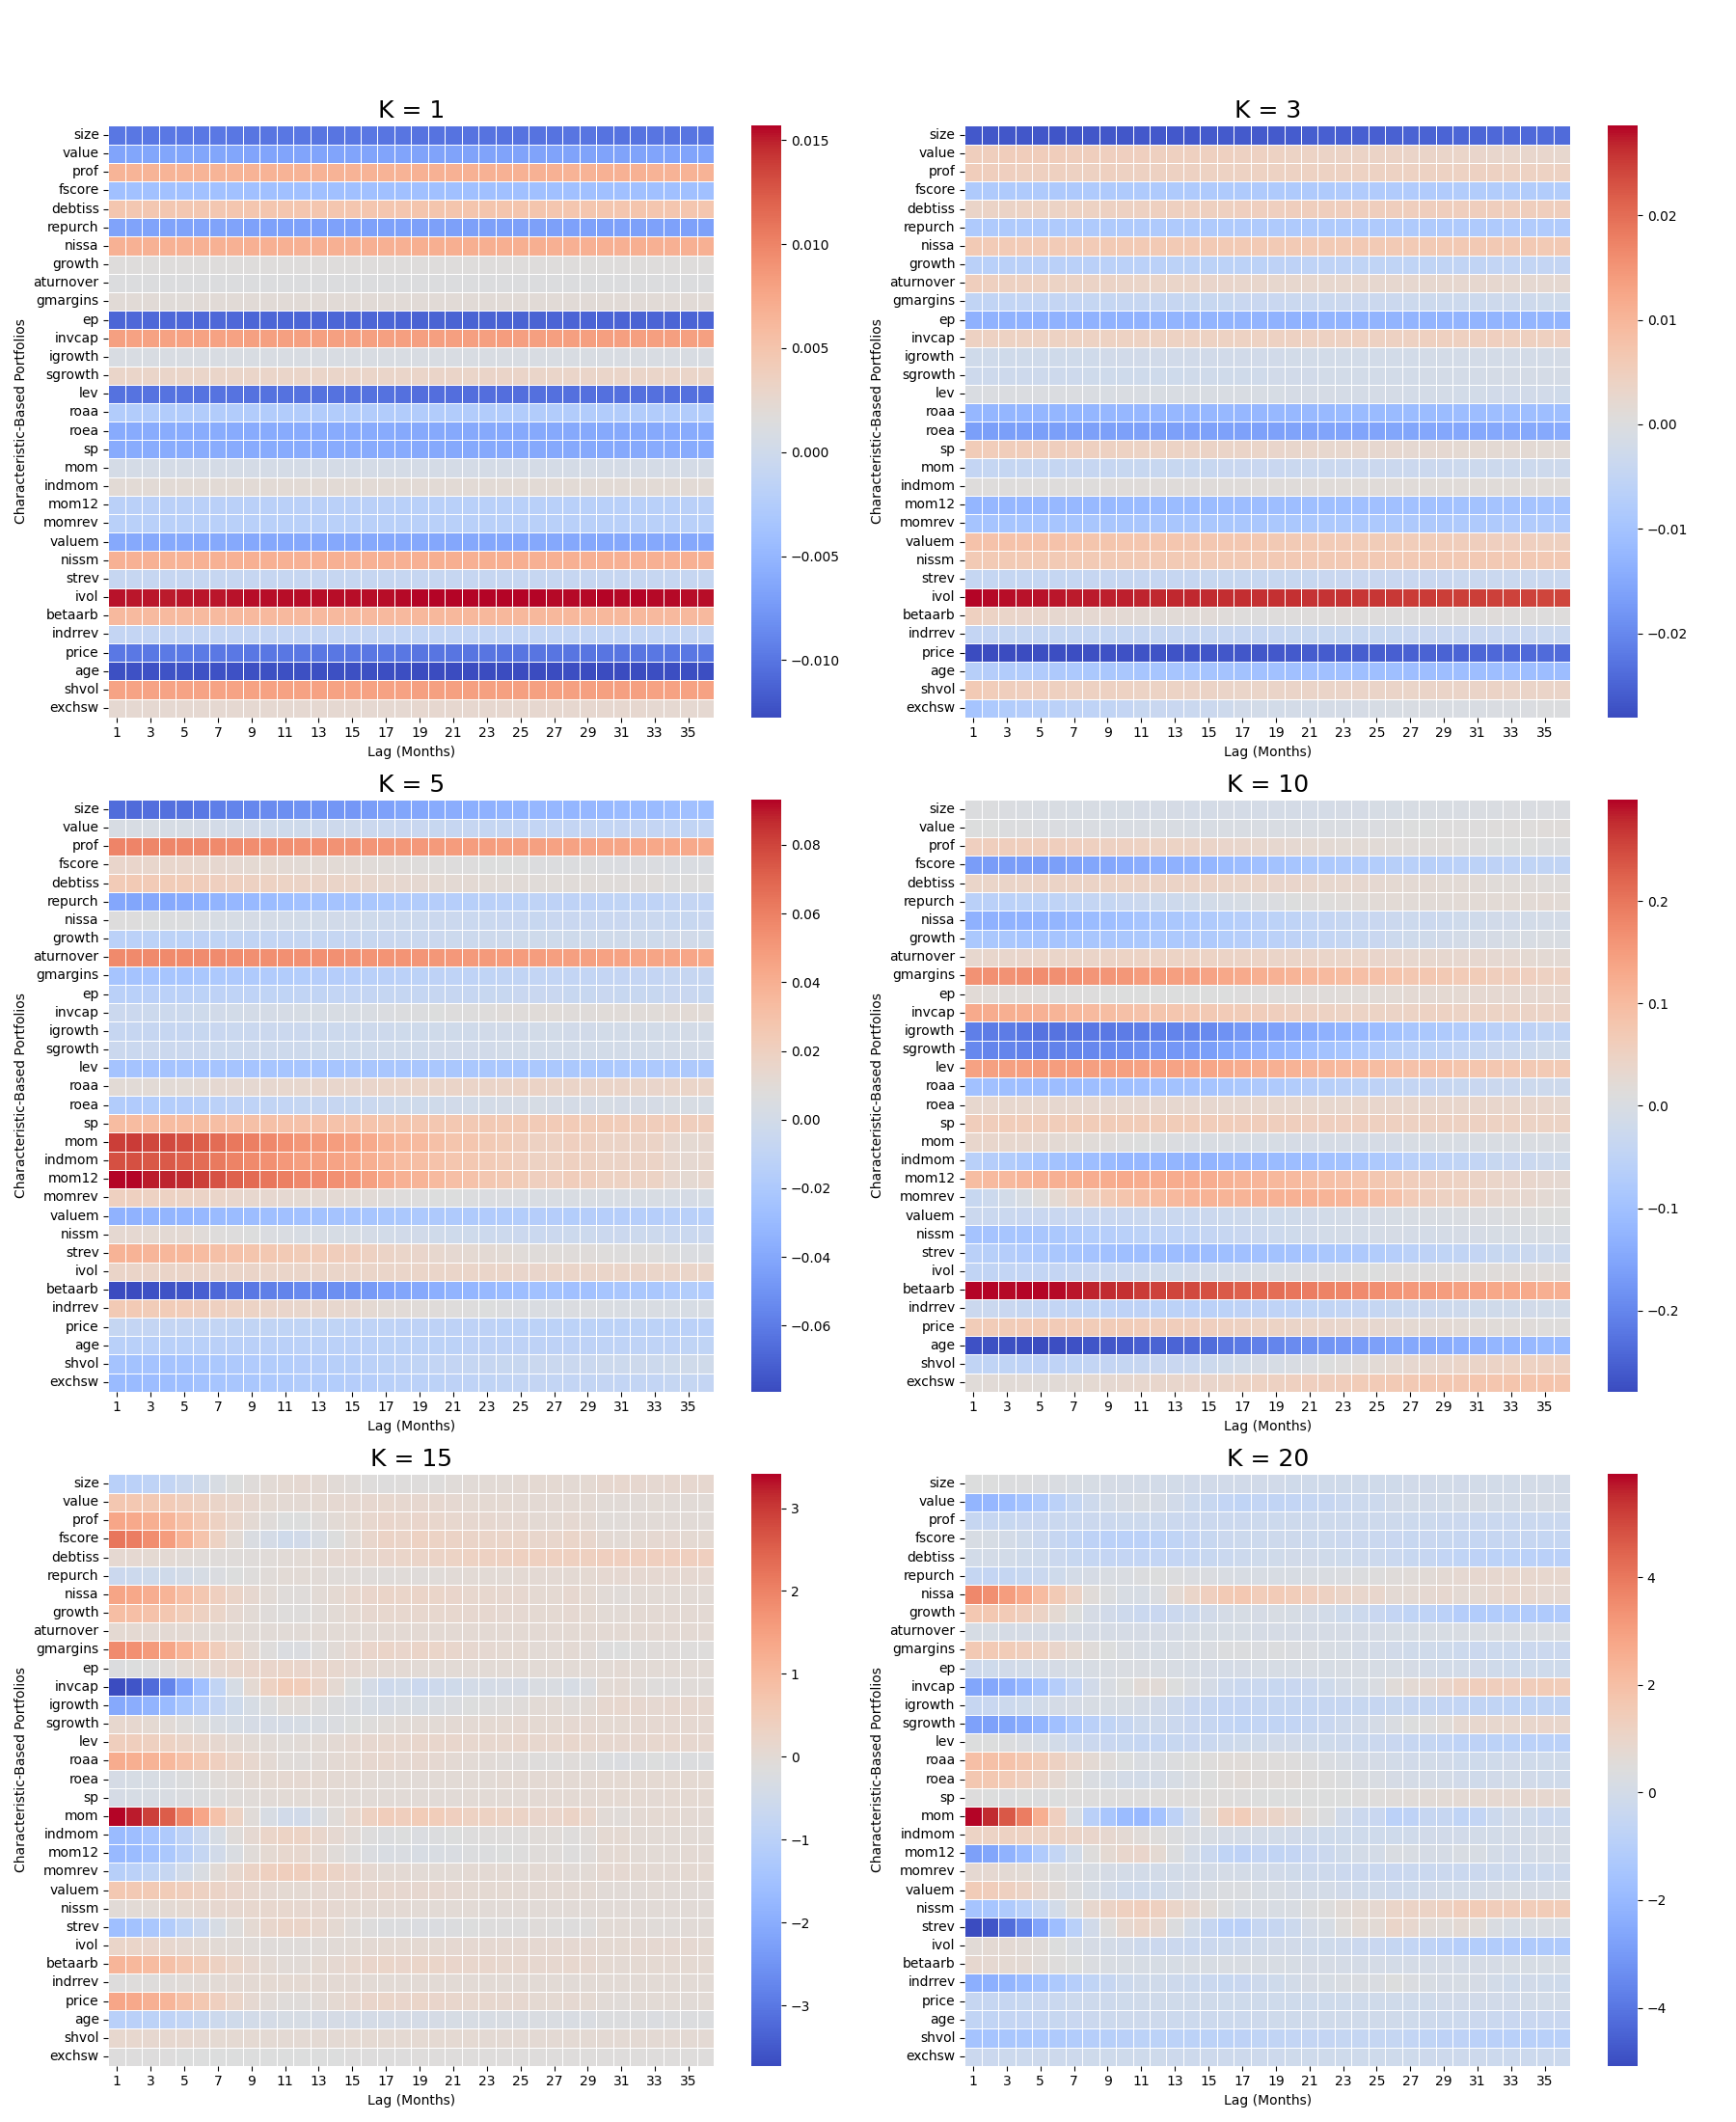
\includegraphics[width=1\linewidth]{WB_36_unnorm.png}
    \caption{Unnormalized Lag Loadings in Portfolio Space, Lag = 36 Months}
    \label{fig:WB_36}
\end{figure}

\begin{itemize}
    \item The magnitude of portfolio's lag loadings increases as $K$ increases. 
    \item $K =1$ and $K =3$ appear similar, not much change over lags but largest magnitude chars are 
    idiosyncratic volatility, size, price and age - still small magnitude though
    \item Medium-size models start to show weight decay as lags increase; $K = 5$ loads heavily on momentum factors, 
    negative loading on size and beta arbitrage.$K = 10$ loads positively on beta arbitrage and less so on momentum, but also heavily on 
    sales growth and investment growth.
    \item Larger models re-load back on momentum
\end{itemize}

\begin{figure}[H]
    \centering
    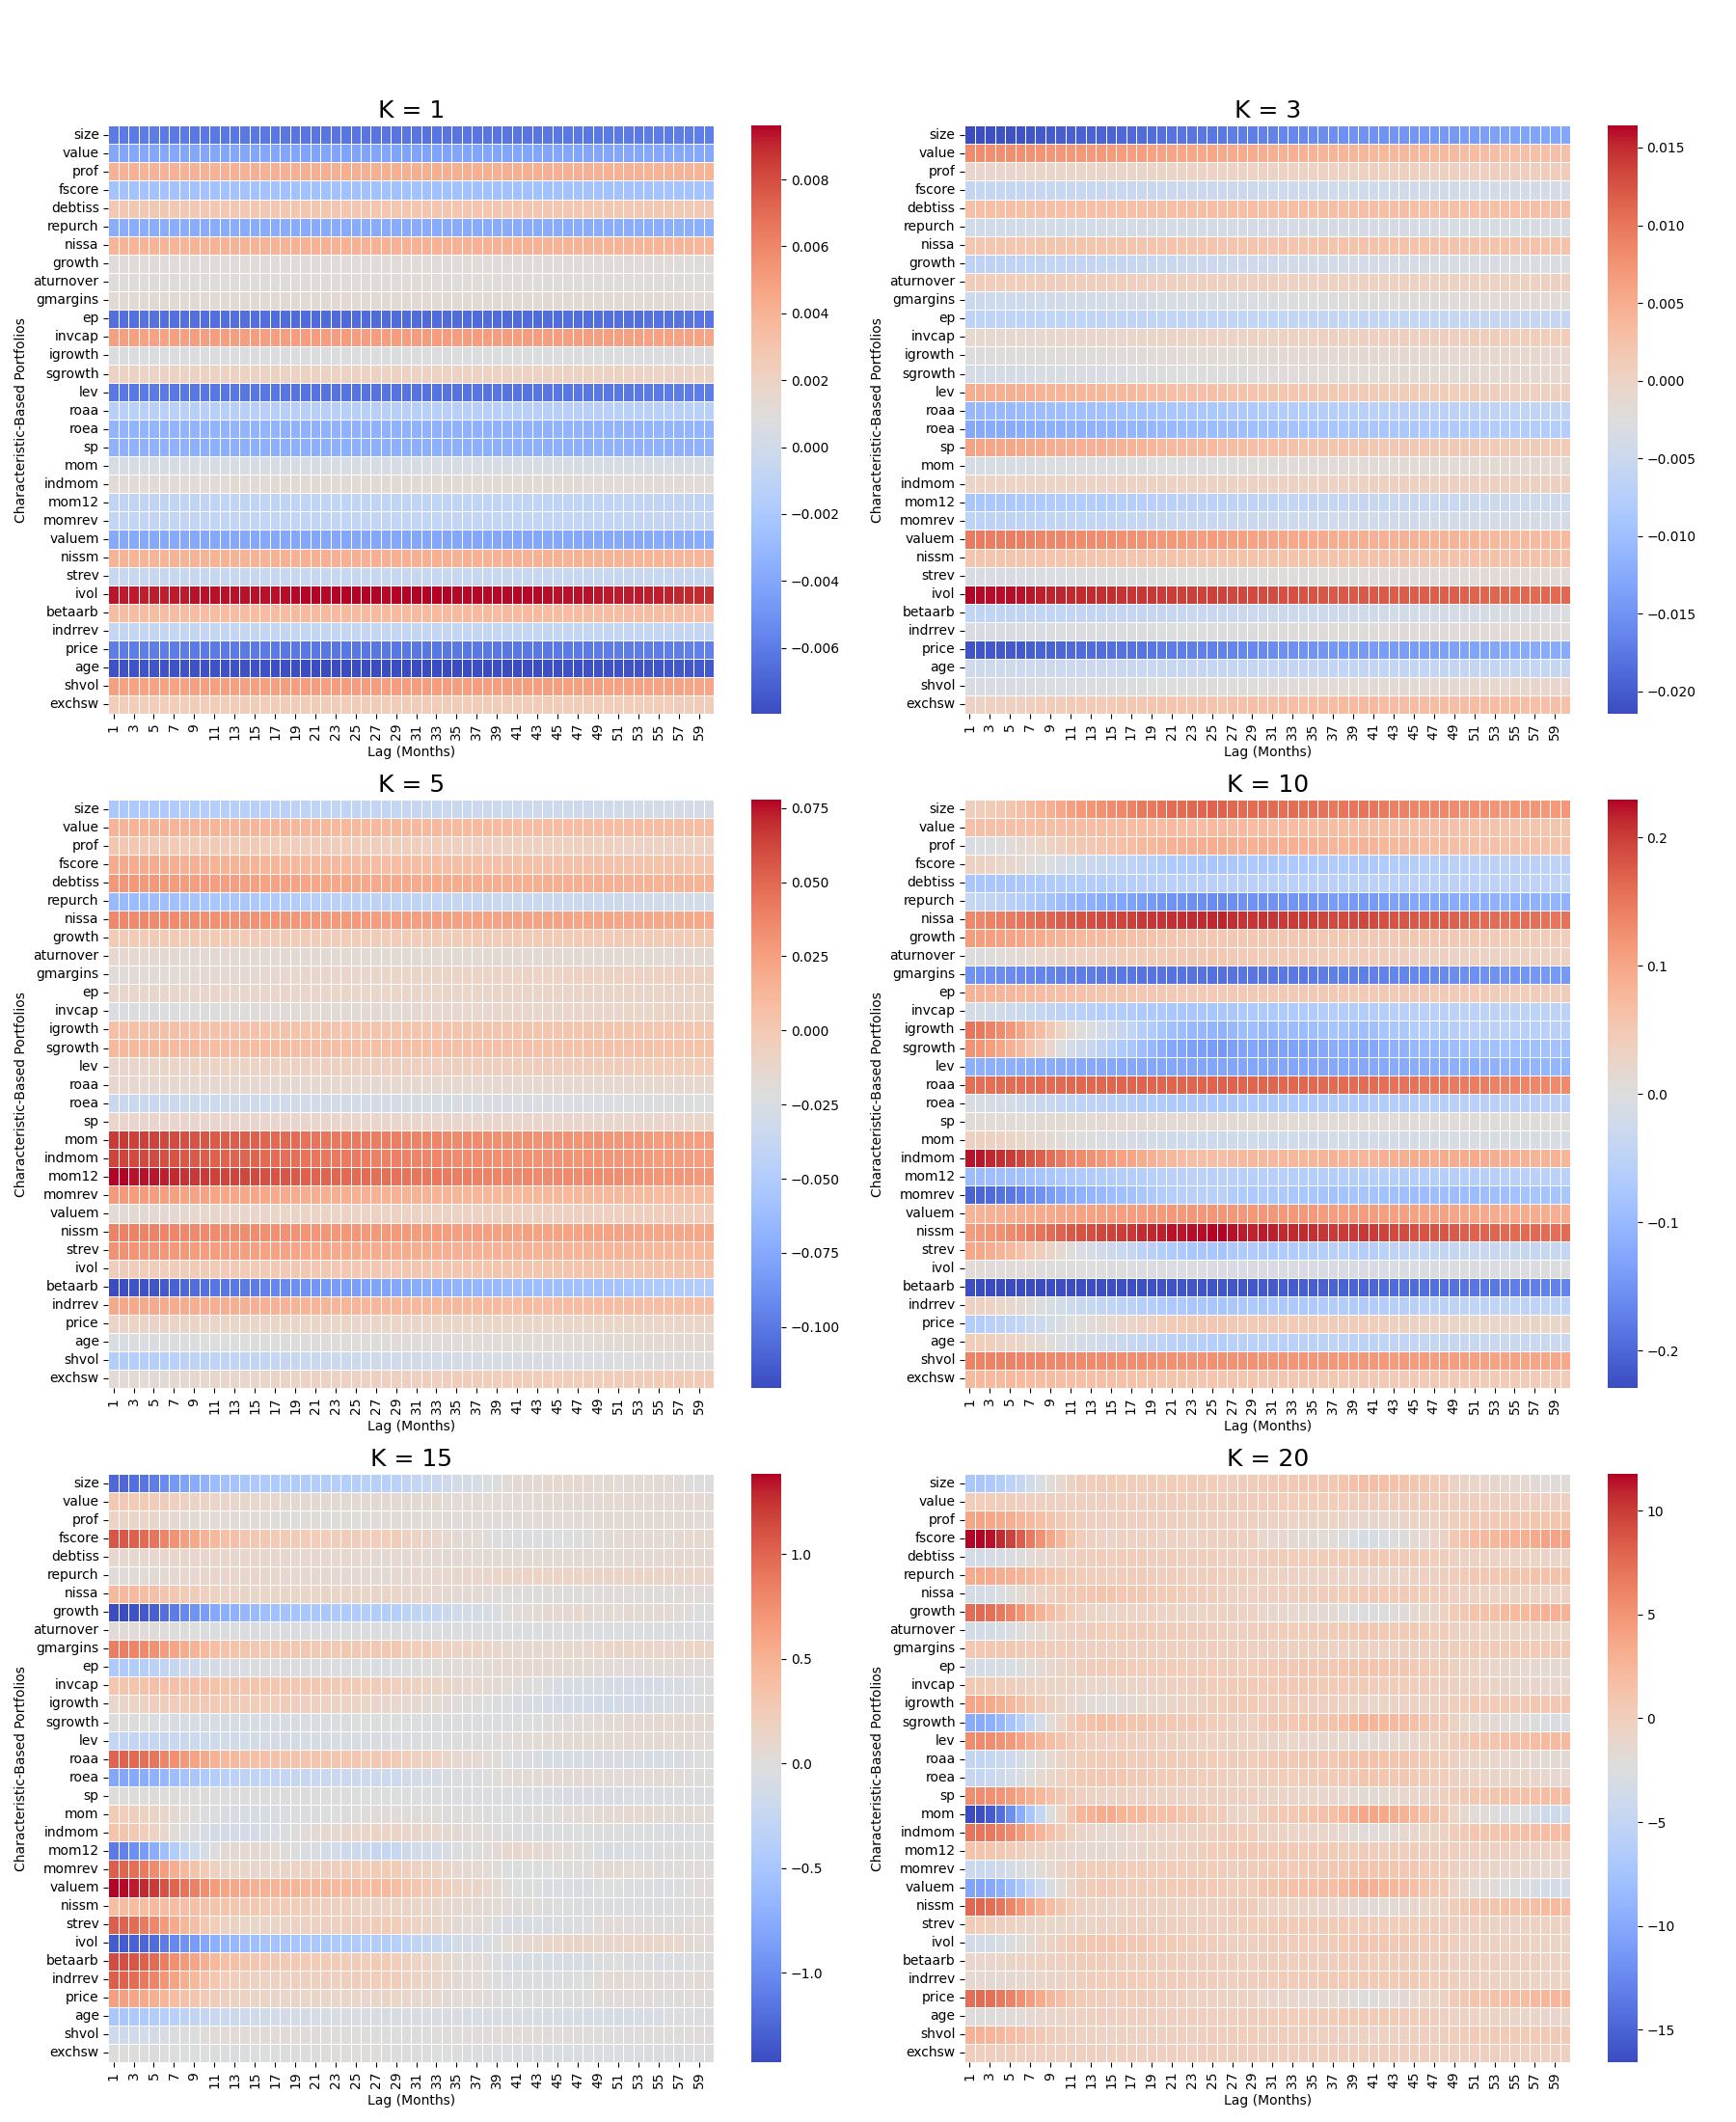
\includegraphics[width=1\linewidth]{WB_60_unnorm.png}
    \caption{Unnormalized Lag Loadings in Portfolio Space, Lag = 60 Months}
    \label{fig:WB_60}
\end{figure}

\begin{itemize}
    \item A similar story for the smaller models
    \item Somewhat similar for medium models; $K = 5$ loads positively on momentum portfolios and negatively on betaarb; 
    $K = 10$ is now also negative on beta arb but now captures some more variation in the sales growth 
    and investment growth portfolios (ie. positive to negative rather than strictly negative as before)
\end{itemize}

\begin{figure}[H]
    \centering
    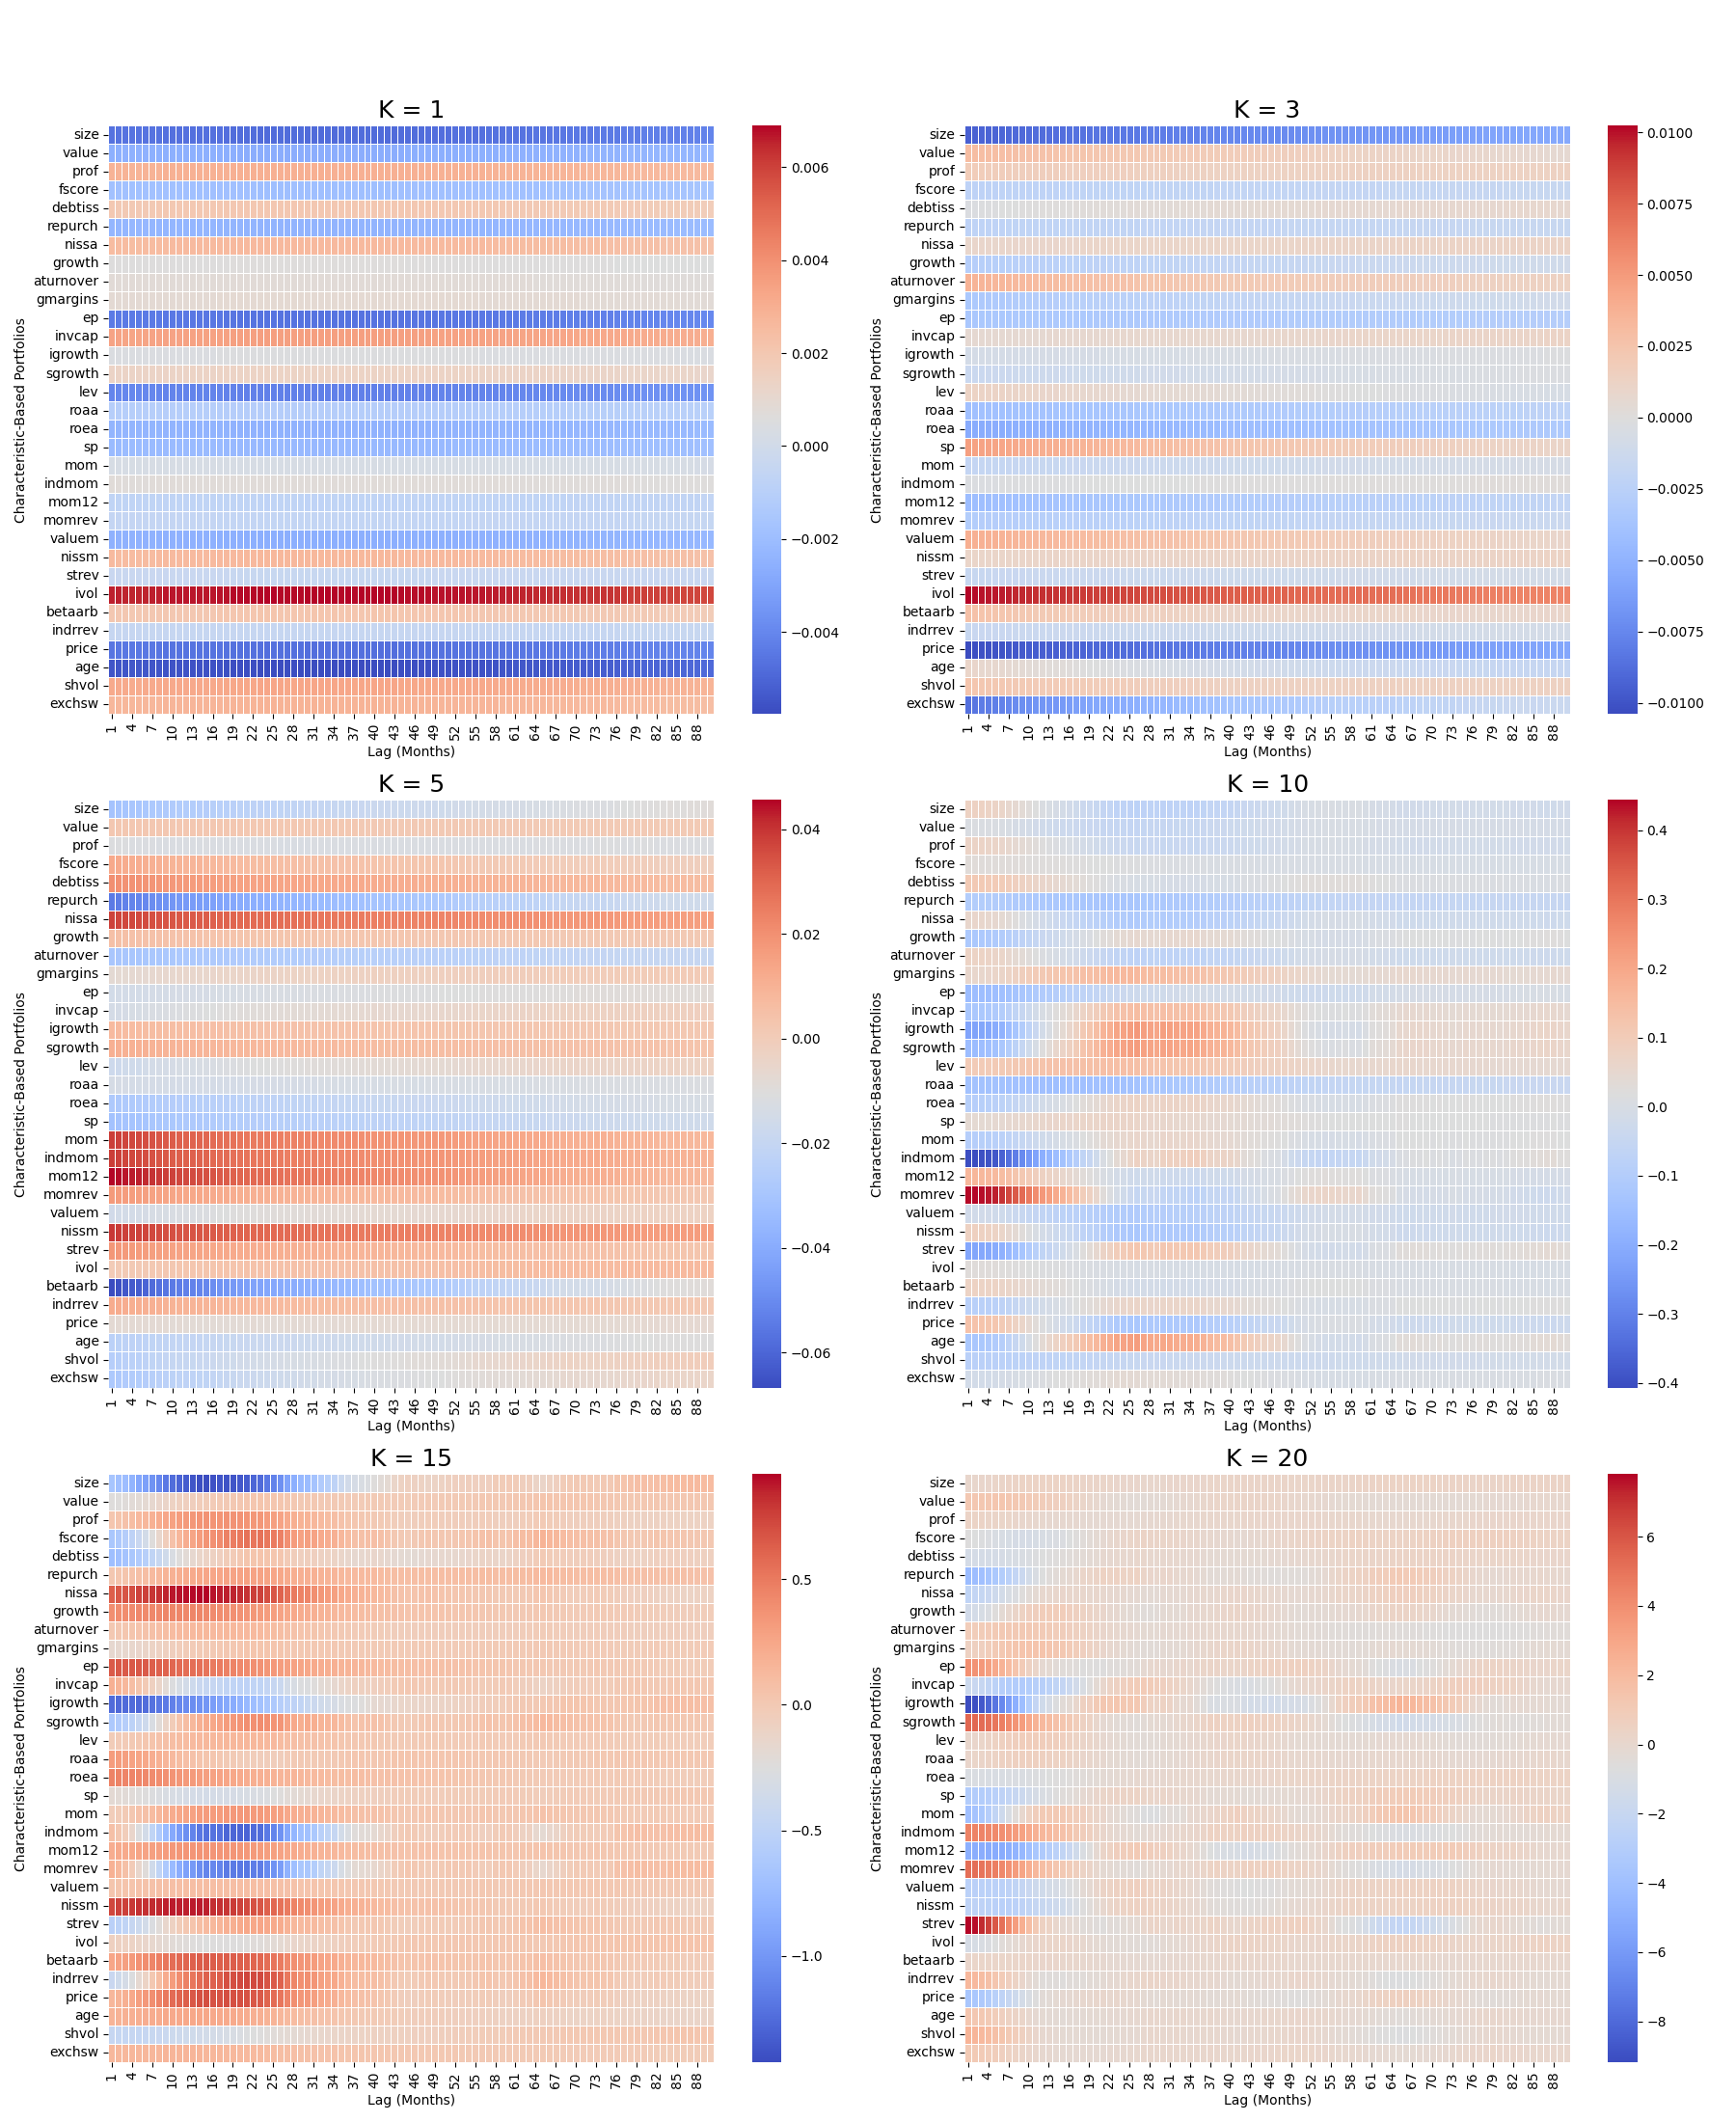
\includegraphics[width=1\linewidth]{WB_90_unnorm.png}
    \caption{Unnormalized Lag Loadings in Portfolio Space, Lag = 90 Months}
    \label{fig:WB_90}
\end{figure}

\begin{figure}[H]
    \centering
    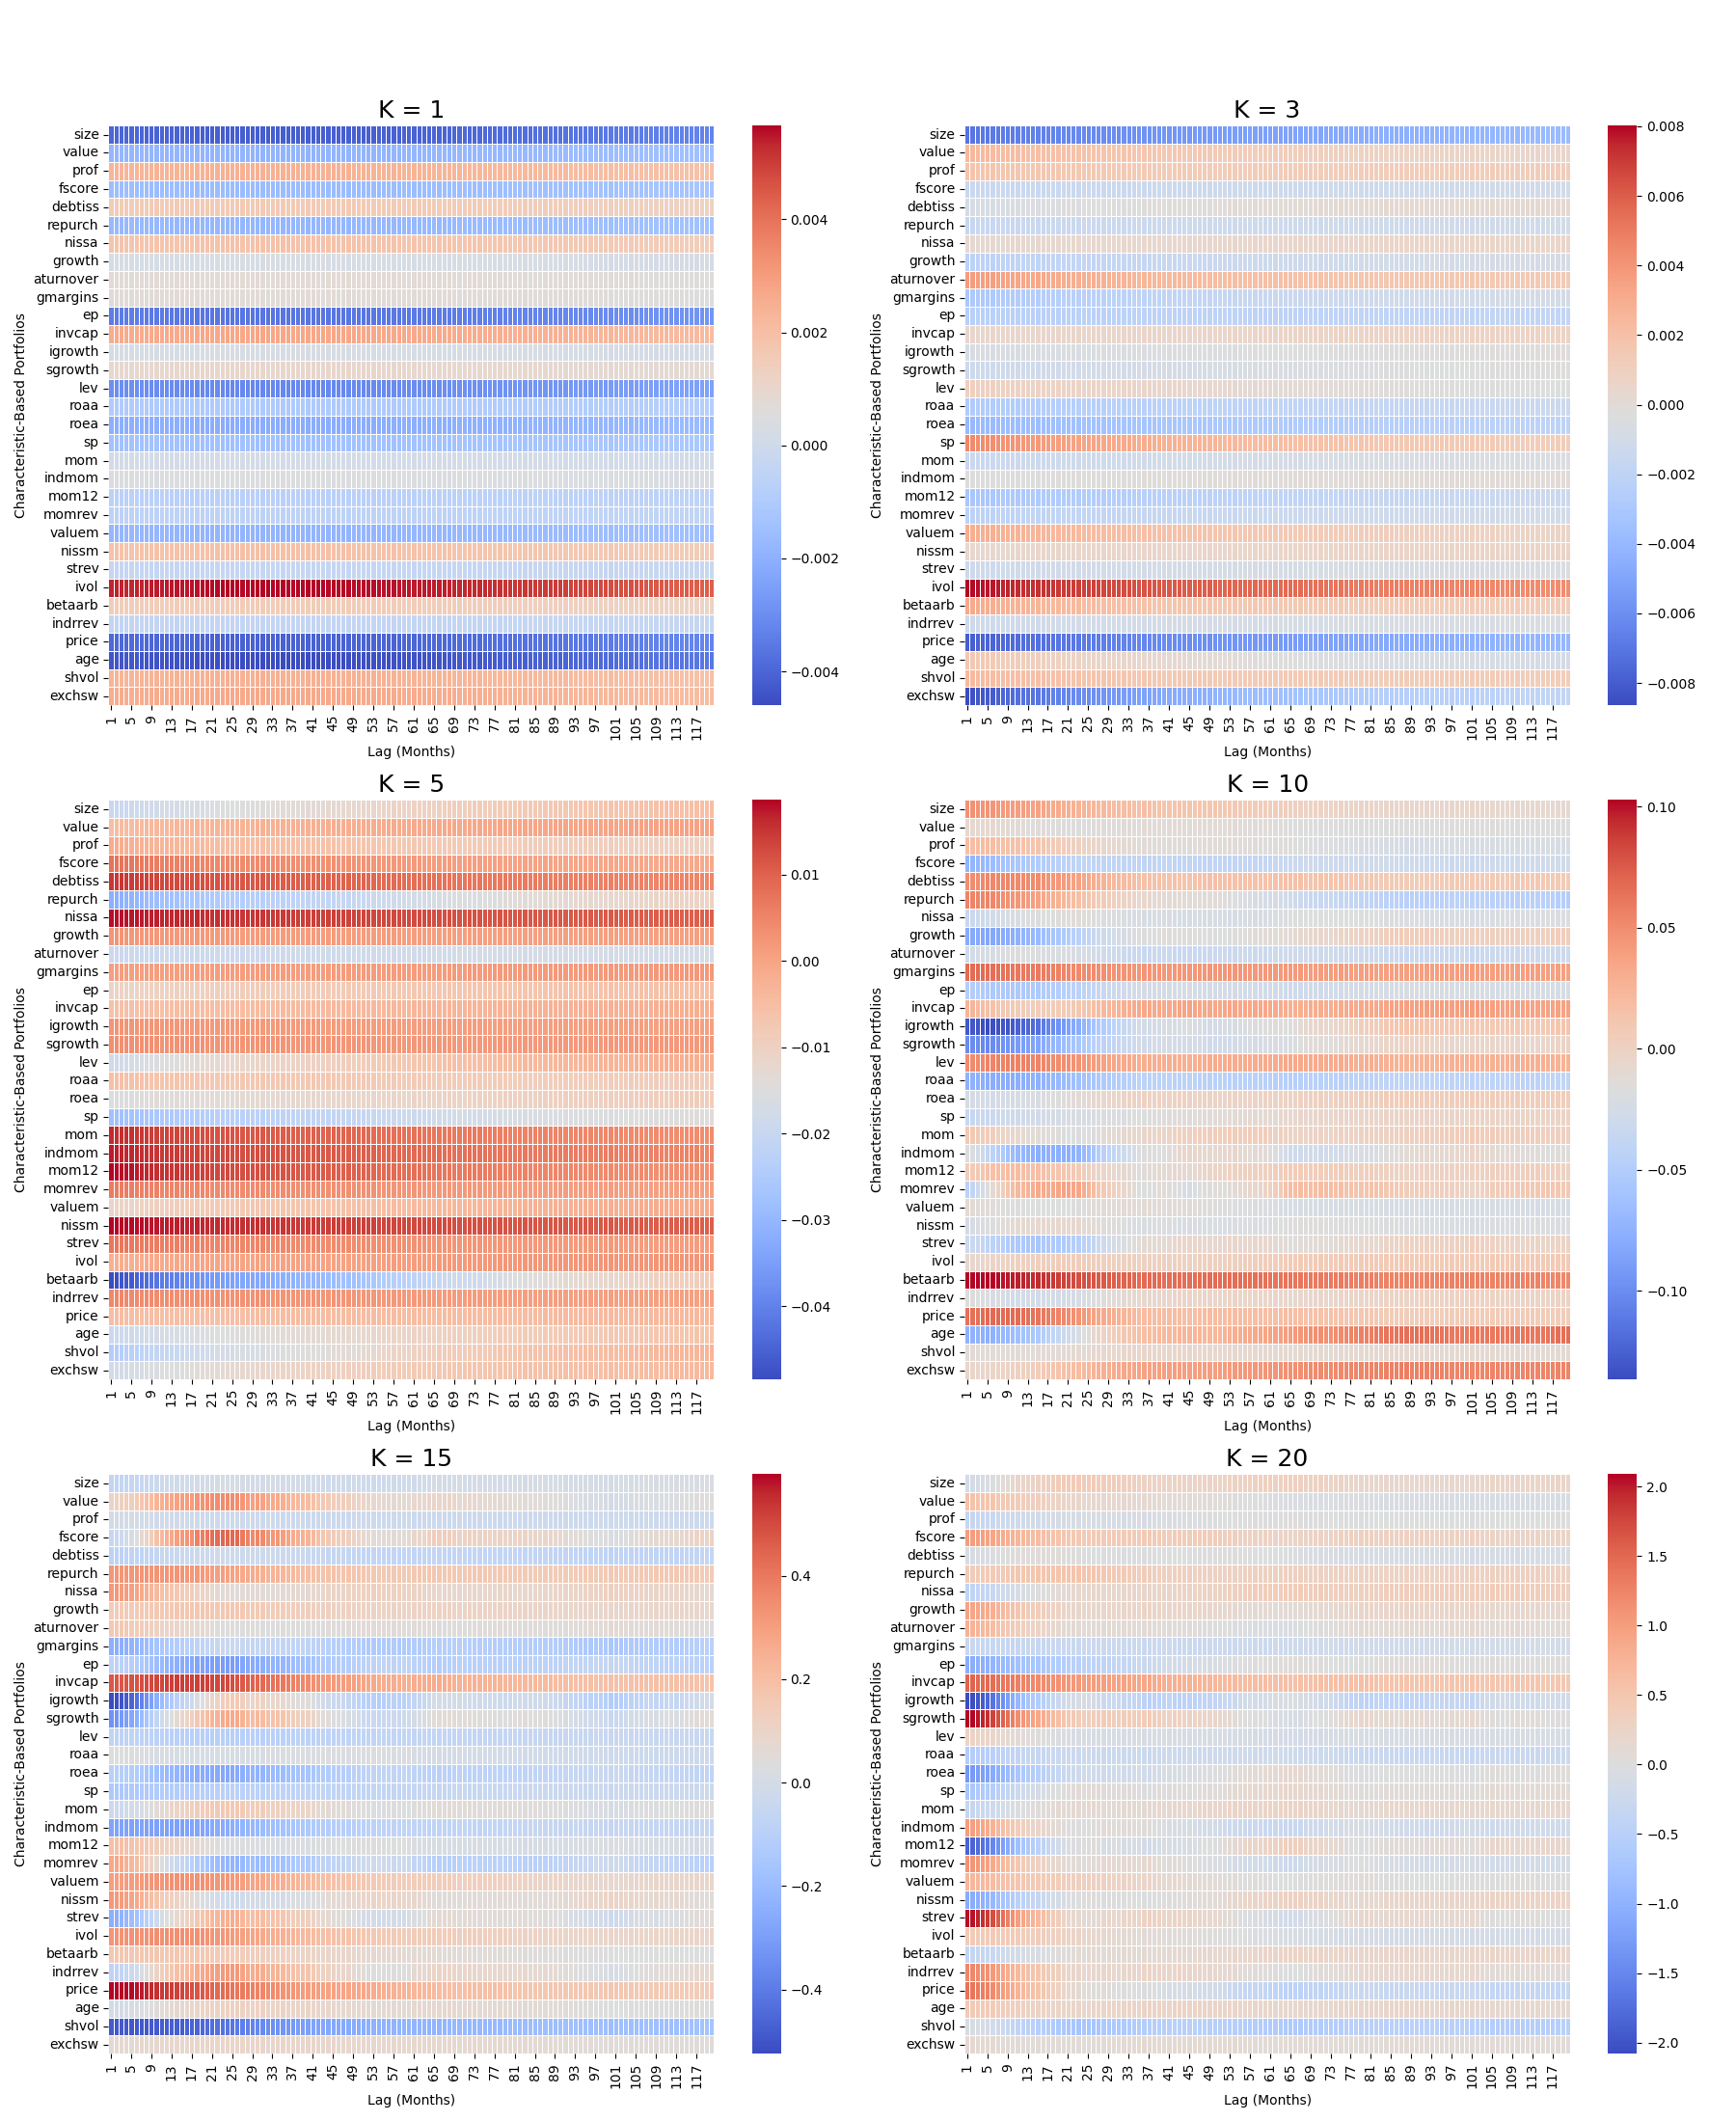
\includegraphics[width=1\linewidth]{WB_120_unnorm.png}
    \caption{Unnormalized Lag Loadings in Portfolio Space, Lag = 120 Months}
    \label{fig:WB_120}
\end{figure}

Note that we can also normalize each of the lag loadings in portfolio space such that 
each characteristic has unit norm across lags. This way, we can better understand how each 
characteristic's loading dynamics as a function of lags, rather than just the largest magnitudes. 
To ensure equality in the tensor factor model, the scalar terms can 
subsume the norm. 

\begin{figure}[H]
    \centering
    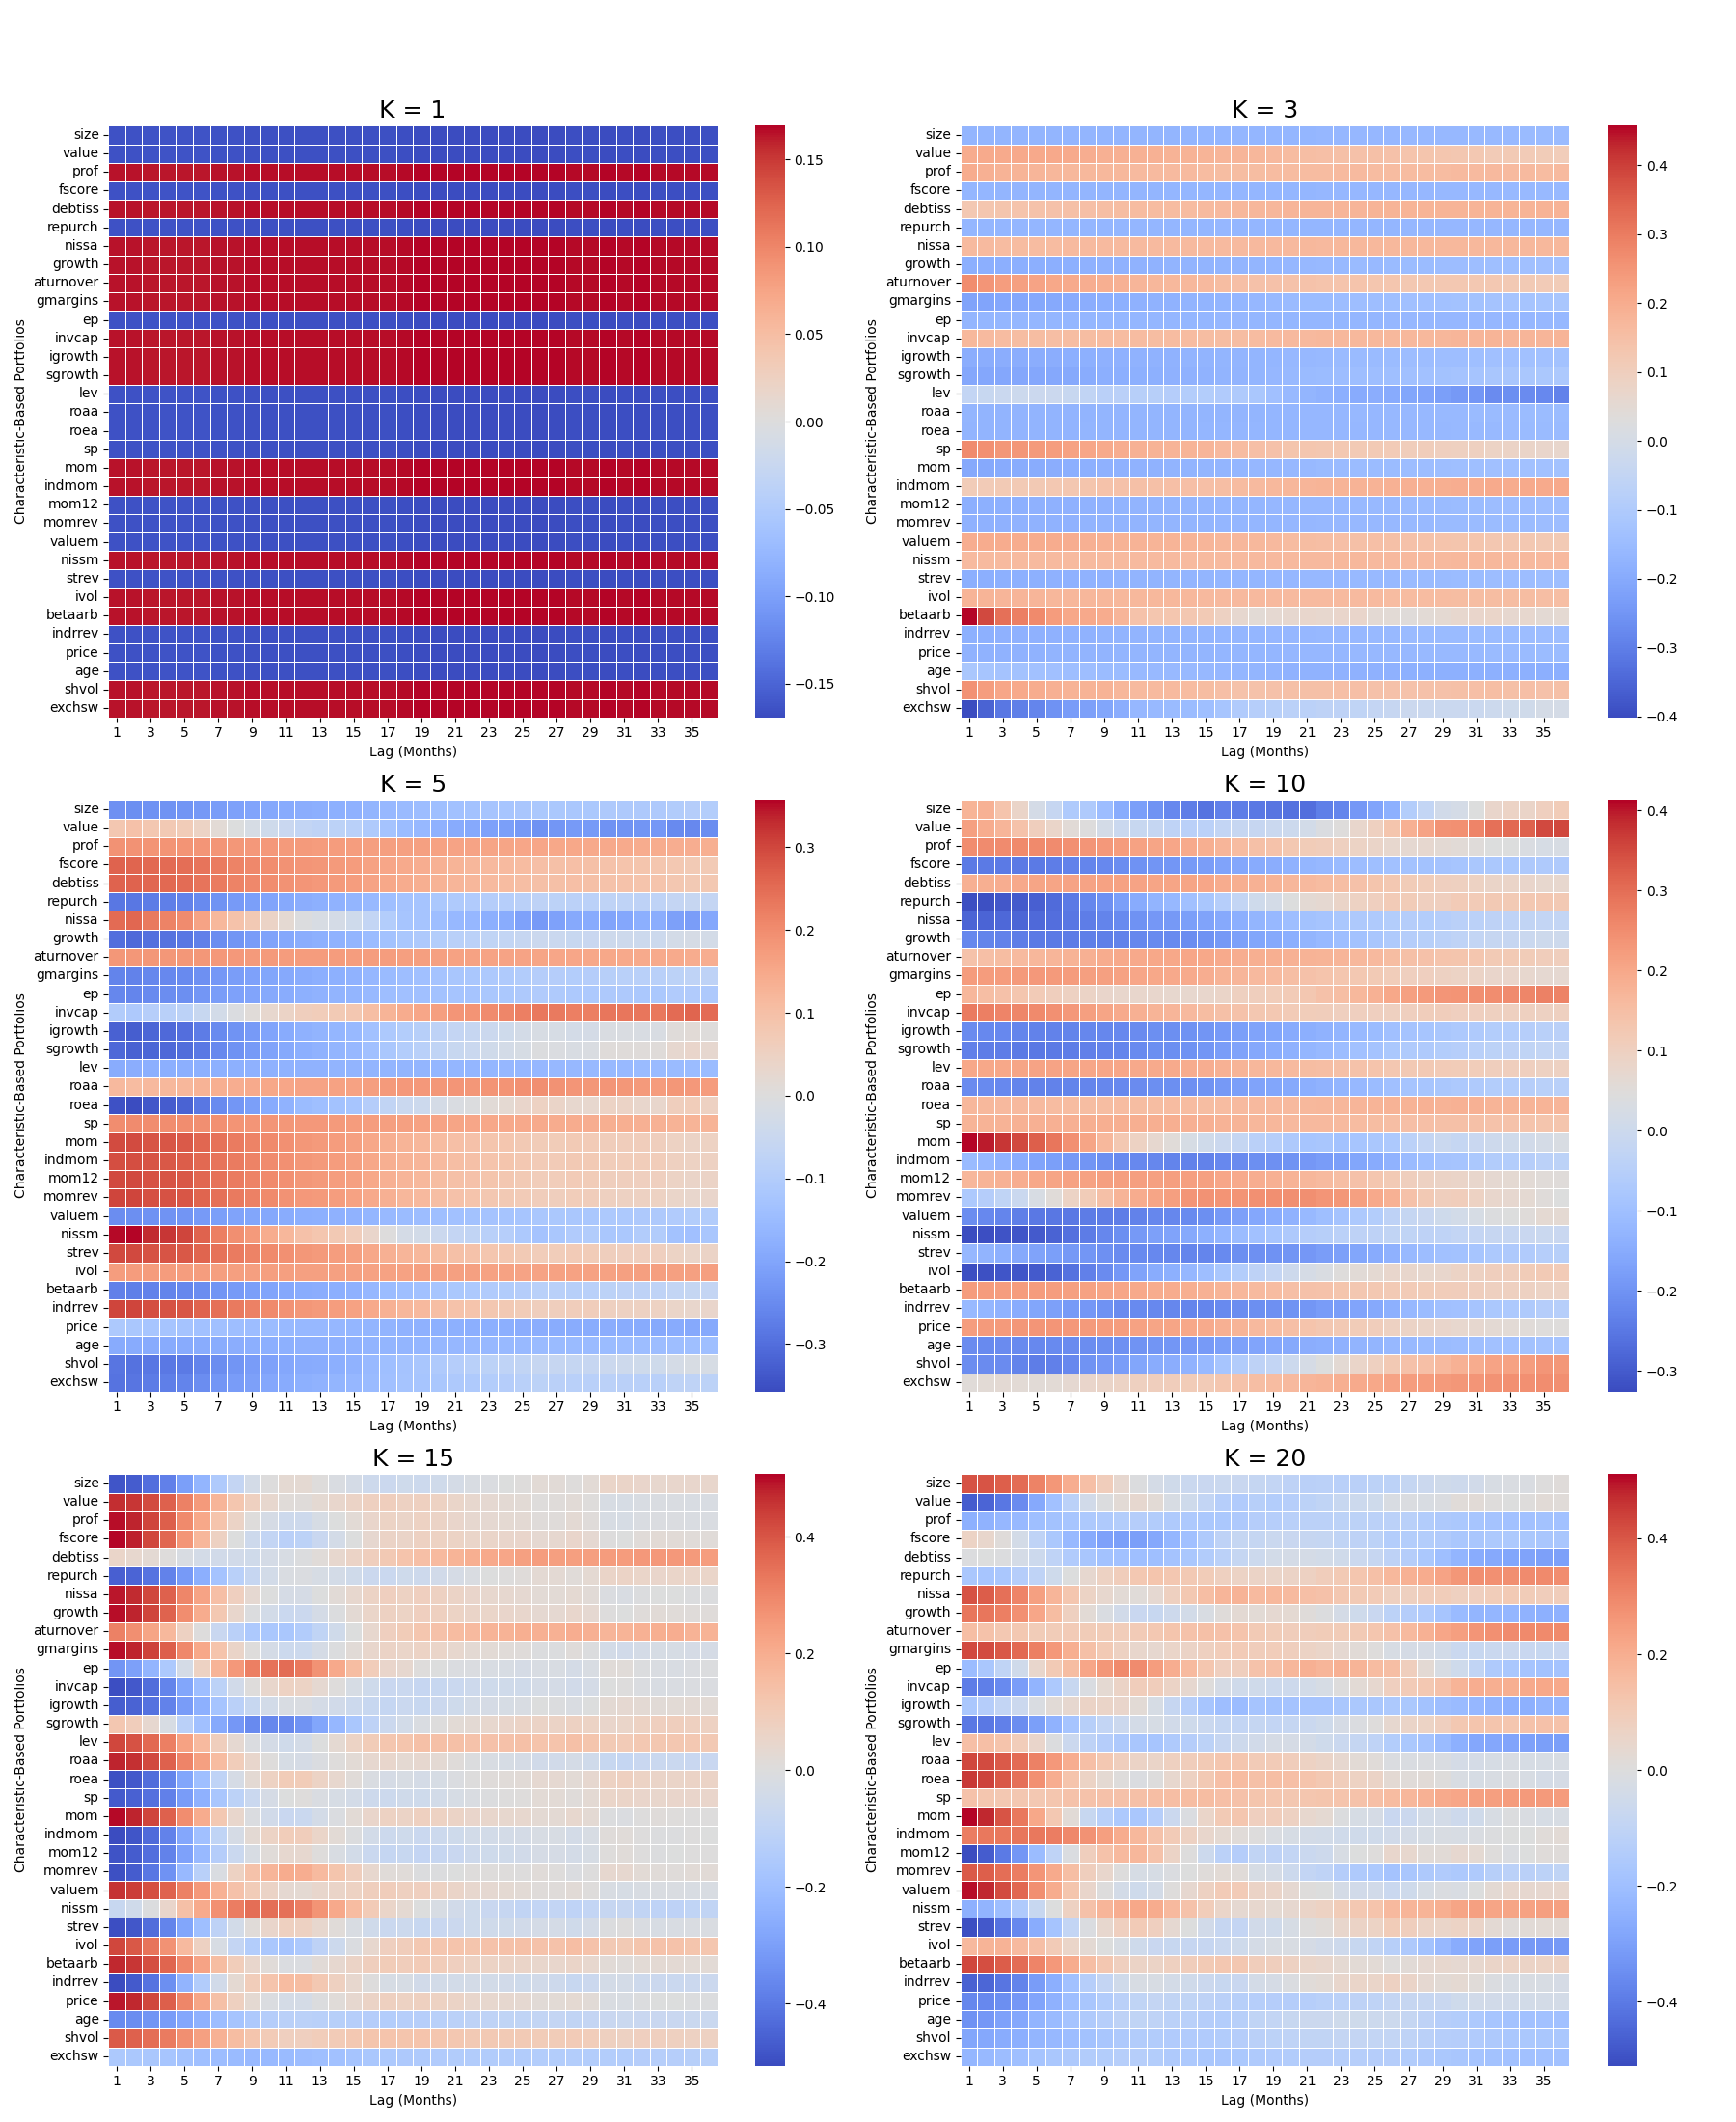
\includegraphics[width=1\linewidth]{WB_36_norm.png}
    \caption{Normalized Lag Loadings in Portfolio Space, Lag = 36 Months}
    \label{fig:WB_36_norm}
\end{figure}

\begin{figure}[H]
    \centering
    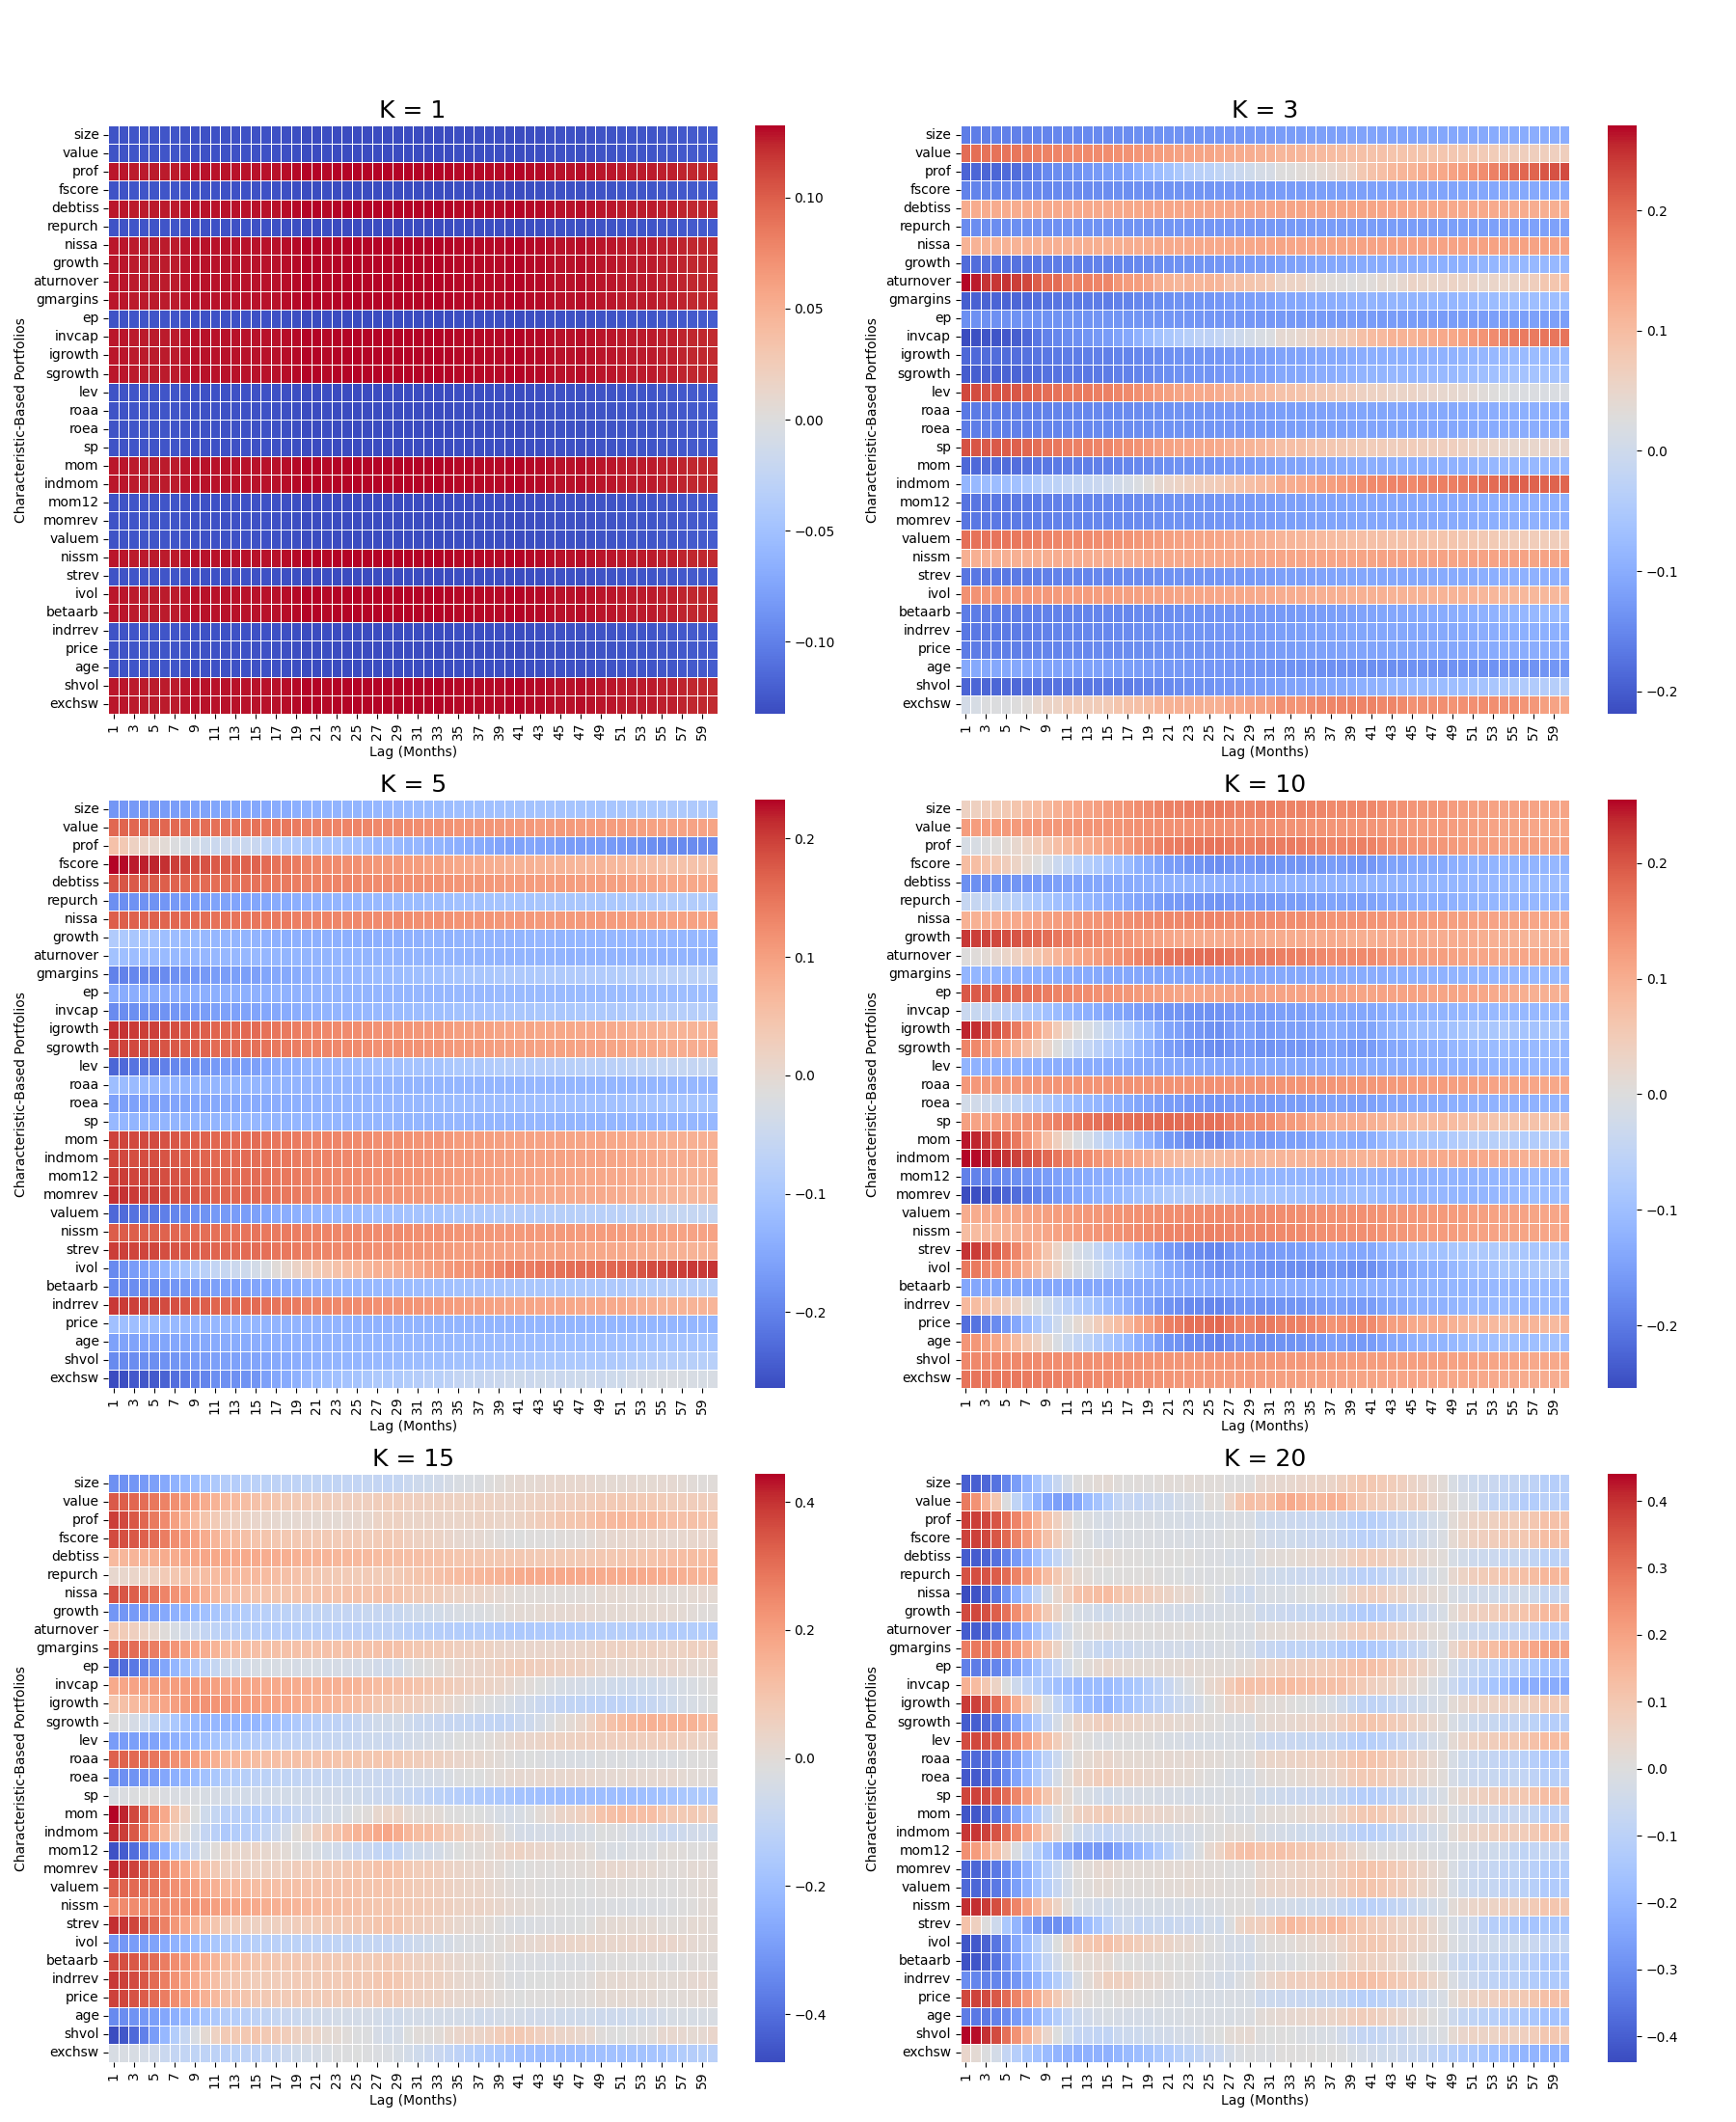
\includegraphics[width=1\linewidth]{WB_60_norm.png}
    \caption{Normalized Lag Loadings in Portfolio Space, Lag = 60 Months}
    \label{fig:WB_60_norm}
\end{figure}

\begin{figure}[H]
    \centering
    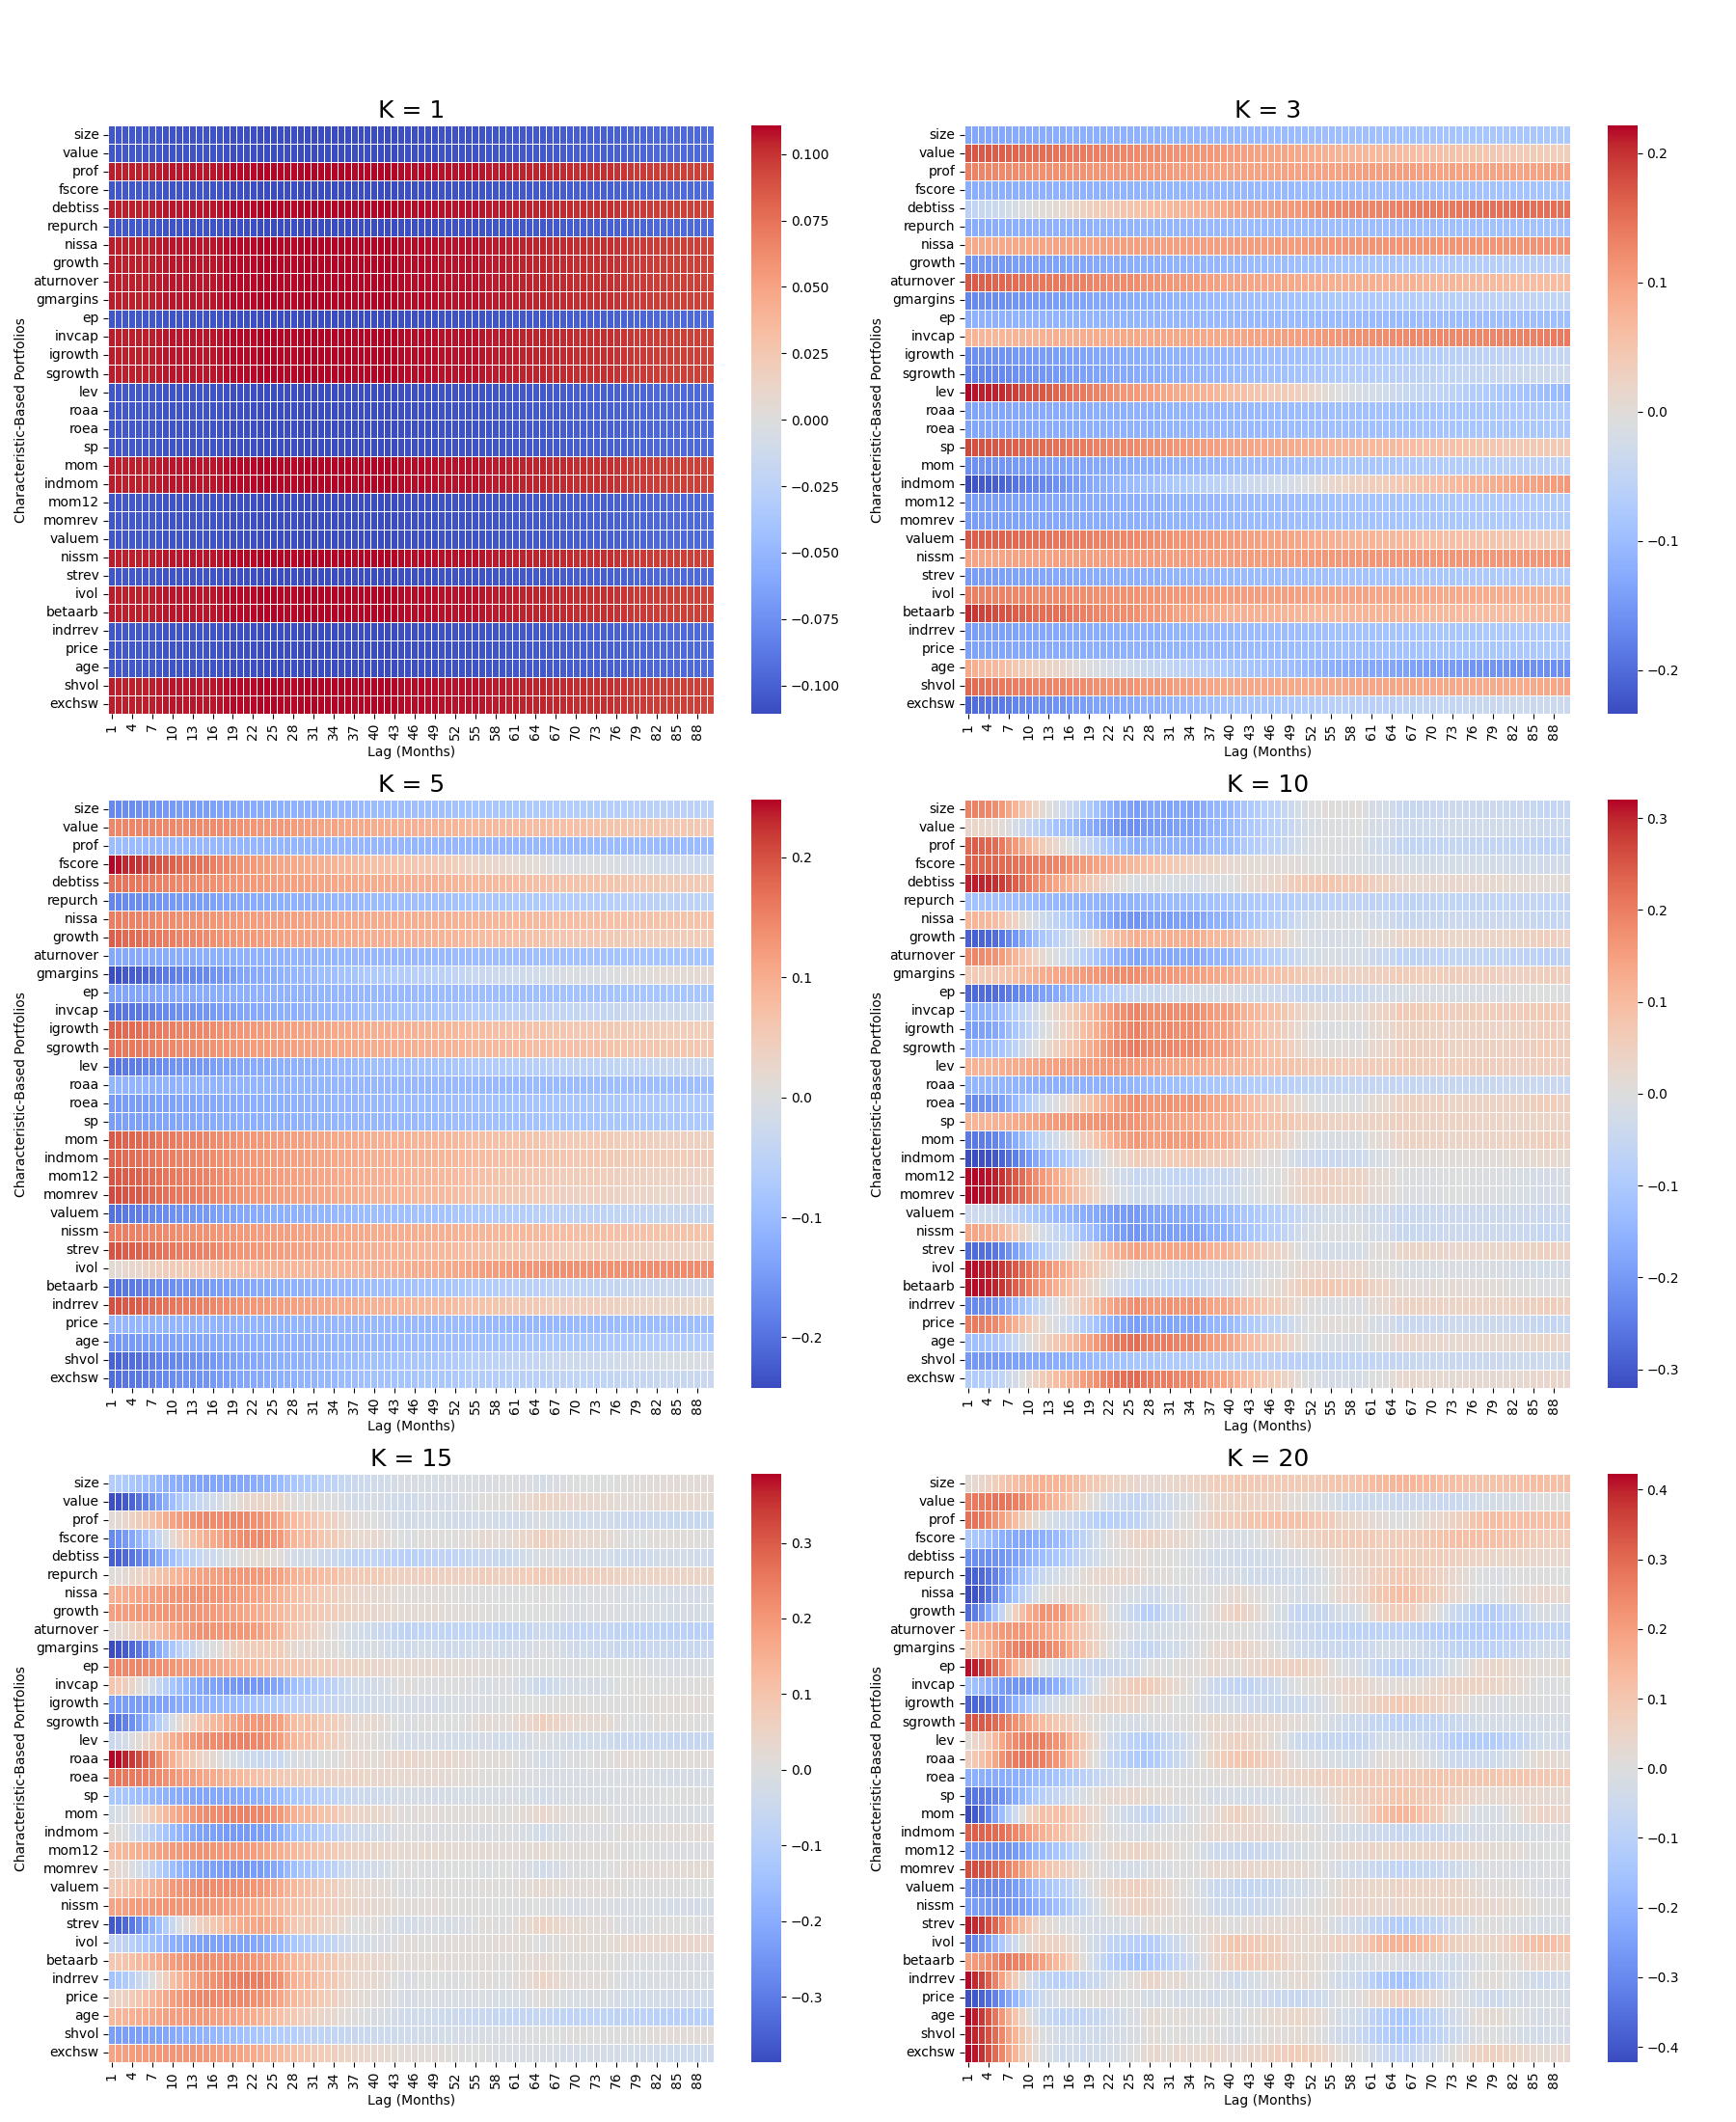
\includegraphics[width=1\linewidth]{WB_90_norm.png}
    \caption{Normalized Lag Loadings in Portfolio Space, Lag = 90 Months}
    \label{fig:WB_90_norm}
\end{figure}

\begin{figure}[H]
    \centering
    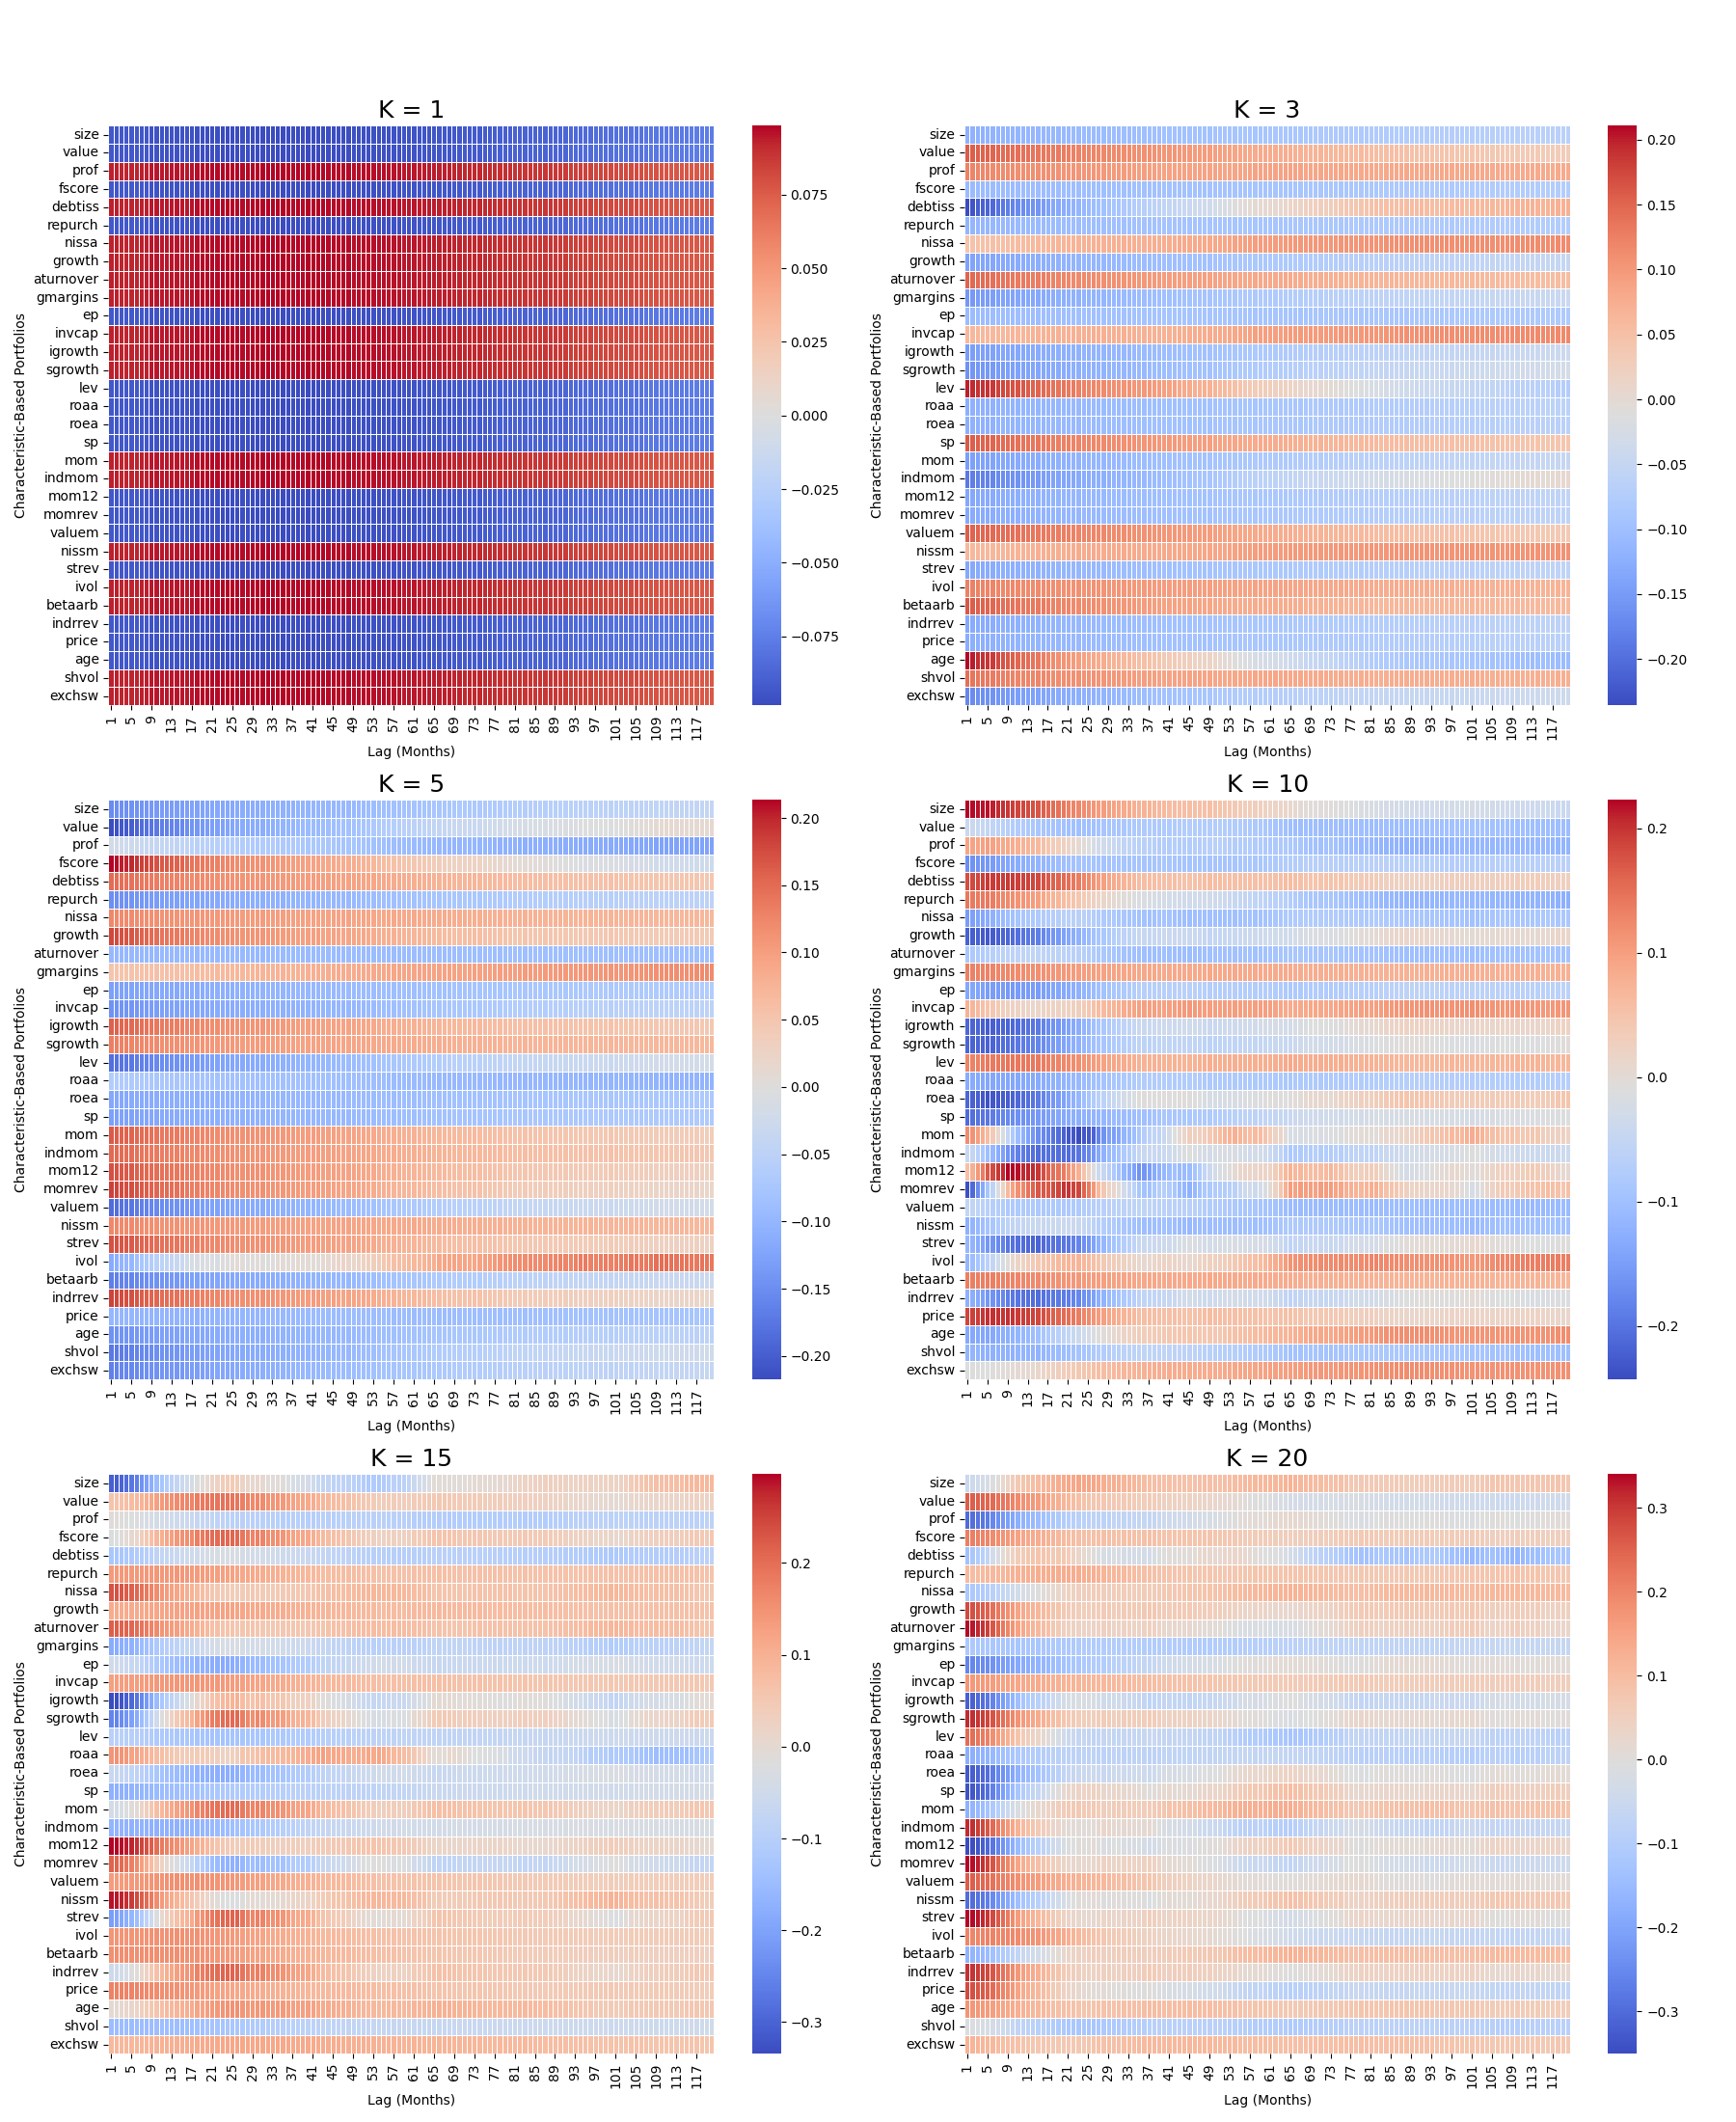
\includegraphics[width=1\linewidth]{WB_120_norm.png}
    \caption{Normalized Lag Loadings in Portfolio Space, Lag = 120 Months}
    \label{fig:WB_120_norm}
\end{figure}

Questions that we want to answer
\begin{itemize}
    \item Generally, which characteristics load on small lags and which load on long lags?
    \item How do these lag loadings change as a function of lags?
    \item How do these lag loadings change as a function of $K$?
\end{itemize}

However, since certain characteristics weights decay are not stable over time, 
these plots can be slightly misleading. If we impose some regularization or ridge regression on $\bm{W}$, 
could these stabilize over time without sacrificing performance? See \verb|interp.ipynb| 
notebook for these graphs for one arbitrary local instance (120-month rolling window).

\subsection{Sparsity (and Other Regularizations) in PARAFAC}
\begin{itemize}
    \item Maybe L1 on $\bm{W} \implies$ after implementing this, we could try testing to see if this leads to higher multihorizon Sharpe Ratios 
    \item Also with L1 implemented, are the local $\bm{W}$'s more highly correlated, but the global model should also be sparse right?
    \item NOTE: it's actually problematic to perform soft-thresholding (L1 regularization) during ALS. It also doesn't work too well to 
    apply it to the ALS output (traditional Lasso), and the solution in the literature is to forget ALS and instead work with 
    an alternating proximal gradient. \verb|Tensorly| has implemented this, shouldn't be too bad for us to implement. 
    \item No obvious PCA comparison, obviously
\end{itemize}

\section{Notes, 3/10}

Bigger picture
\begin{itemize}
    \item 
\end{itemize}

\end{document}
